% Template for PLoS
% Version 3.5 March 2018
%
% % % % % % % % % % % % % % % % % % % % % %
%
% -- IMPORTANT NOTE
%
% This template contains comments intended 
% to minimize problems and delays during our production 
% process. Please follow the template instructions
% whenever possible.
%
% % % % % % % % % % % % % % % % % % % % % % % 
%
% Once your paper is accepted for publication, 
% PLEASE REMOVE ALL TRACKED CHANGES in this file 
% and leave only the final text of your manuscript. 
% PLOS recommends the use of latexdiff to track changes during review, as this will help to maintain a clean tex file.
% Visit https://www.ctan.org/pkg/latexdiff?lang=en for info or contact us at latex@plos.org.
%
%
% There are no restrictions on package use within the LaTeX files except that 
% no packages listed in the template may be deleted.
%
% Please do not include colors or graphics in the text.
%
% The manuscript LaTeX source should be contained within a single file (do not use \input, \externaldocument, or similar commands).
%
% % % % % % % % % % % % % % % % % % % % % % %
%
% -- FIGURES AND TABLES
%
% Please include tables/figure captions directly after the paragraph where they are first cited in the text.
%
% DO NOT INCLUDE GRAPHICS IN YOUR MANUSCRIPT
% - Figures should be uploaded separately from your manuscript file. 
% - Figures generated using LaTeX should be extracted and removed from the PDF before submission. 
% - Figures containing multiple panels/subfigures must be combined into one image file before submission.
% For figure citations, please use "Fig" instead of "Figure".
% See http://journals.plos.org/plosone/s/figures for PLOS figure guidelines.
%
% Tables should be cell-based and may not contain:
% - spacing/line breaks within cells to alter layout or alignment
% - do not nest tabular environments (no tabular environments within tabular environments)
% - no graphics or colored text (cell background color/shading OK)
% See http://journals.plos.org/plosone/s/tables for table guidelines.
%
% For tables that exceed the width of the text column, use the adjustwidth environment as illustrated in the example table in text below.
%
% % % % % % % % % % % % % % % % % % % % % % % %
%
% -- EQUATIONS, MATH SYMBOLS, SUBSCRIPTS, AND SUPERSCRIPTS
%
% IMPORTANT
% Below are a few tips to help format your equations and other special characters according to our specifications. For more tips to help reduce the possibility of formatting errors during conversion, please see our LaTeX guidelines at http://journals.plos.org/plosone/s/latex
%
% For inline equations, please be sure to include all portions of an equation in the math environment.  For example, x$^2$ is incorrect; this should be formatted as $x^2$ (or $\mathrm{x}^2$ if the romanized font is desired).
%
% Do not include text that is not math in the math environment. For example, CO2 should be written as CO\textsubscript{2} instead of CO$_2$.
%
% Please add line breaks to long display equations when possible in order to fit size of the column. 
%
% For inline equations, please do not include punctuation (commas, etc) within the math environment unless this is part of the equation.
%
% When adding superscript or subscripts outside of brackets/braces, please group using {}.  For example, change "[U(D,E,\gamma)]^2" to "{[U(D,E,\gamma)]}^2". 
%
% Do not use \cal for caligraphic font.  Instead, use \mathcal{}
%
% % % % % % % % % % % % % % % % % % % % % % % % 
%
% Please contact latex@plos.org with any questions.
%
% % % % % % % % % % % % % % % % % % % % % % % %

\documentclass[10pt,letterpaper]{article}
\usepackage[top=0.85in,left=2.75in,footskip=0.75in]{geometry}

% amsmath and amssymb packages, useful for mathematical formulas and symbols
\usepackage{amsmath,amssymb}

% Use adjustwidth environment to exceed column width (see example table in text)
\usepackage{changepage}

% Use Unicode characters when possible
\usepackage[utf8x]{inputenc}

% textcomp package and marvosym package for additional characters
\usepackage{textcomp,marvosym}

% cite package, to clean up citations in the main text. Do not remove.
\usepackage{cite}

% Use nameref to cite supporting information files (see Supporting Information section for more info)
\usepackage{nameref,hyperref}

% line numbers
\usepackage[right]{lineno}

% ligatures disabled
\usepackage{microtype}
\DisableLigatures[f]{encoding = *, family = * }

% color can be used to apply background shading to table cells only
\usepackage[table]{xcolor}

% array package and thick rules for tables
\usepackage{array}

\usepackage{booktabs}
\usepackage{tabularx}
\usepackage{caption}
\usepackage{subcaption}
\usepackage{placeins}

% create "+" rule type for thick vertical lines
\newcolumntype{+}{!{\vrule width 2pt}}

% create \thickcline for thick horizontal lines of variable length
\newlength\savedwidth
\newcommand\thickcline[1]{%
  \noalign{\global\savedwidth\arrayrulewidth\global\arrayrulewidth 2pt}%
  \cline{#1}%
  \noalign{\vskip\arrayrulewidth}%
  \noalign{\global\arrayrulewidth\savedwidth}%
}

% \thickhline command for thick horizontal lines that span the table
\newcommand\thickhline{\noalign{\global\savedwidth\arrayrulewidth\global\arrayrulewidth 2pt}%
\hline
\noalign{\global\arrayrulewidth\savedwidth}}


% Remove comment for double spacing
%\usepackage{setspace} 
%\doublespacing

% Text layout
\raggedright
\setlength{\parindent}{0.5cm}
\textwidth 5.25in 
\textheight 8.75in

% Bold the 'Figure #' in the caption and separate it from the title/caption with a period
% Captions will be left justified
\usepackage[aboveskip=1pt,labelfont=bf,labelsep=period,justification=raggedright,singlelinecheck=off]{caption}
\renewcommand{\figurename}{Fig}

% Use the PLoS provided BiBTeX style
\bibliographystyle{plos2015}

% Remove brackets from numbering in List of References
\makeatletter
\renewcommand{\@biblabel}[1]{\quad#1.}
\makeatother



% Header and Footer with logo
\usepackage{lastpage,fancyhdr,graphicx}
\usepackage{epstopdf}
%\pagestyle{myheadings}
\pagestyle{fancy}
\fancyhf{}
%\setlength{\headheight}{27.023pt}
%\lhead{\includegraphics[width=2.0in]{PLOS-submission.eps}}
\rfoot{\thepage/\pageref{LastPage}}
\renewcommand{\headrulewidth}{0pt}
\renewcommand{\footrule}{\hrule height 2pt \vspace{2mm}}
\fancyheadoffset[L]{2.25in}
\fancyfootoffset[L]{2.25in}
\lfoot{\today}

%% Include all macros below

\newcommand{\lorem}{{\bf LOREM}}
\newcommand{\ipsum}{{\bf IPSUM}}

\newcolumntype{L}[1]{>{\raggedright\arraybackslash}p{#1}}
\newcolumntype{C}[1]{>{\centering\arraybackslash}p{#1}}
\newcolumntype{R}[1]{>{\raggedleft\arraybackslash}p{#1}}

%% END MACROS SECTION


\begin{document}
\vspace*{0.2in}

% Title must be 250 characters or less.
\begin{flushleft}
{\Large
\textbf\newline{Hydra: a mixture modeling framework for subtyping pediatric cancer cohorts using multimodal gene expression signatures} % Please use "sentence case" for title and headings (capitalize only the first word in a title (or heading), the first word in a subtitle (or subheading), and any proper nouns).
}
\newline
% Insert author names, affiliations and corresponding author email (do not include titles, positions, or degrees).
\\
Jacob Pfeil\textsuperscript{1,2*},
Lauren M. Sanders\textsuperscript{1,2,3},
Ioannis Anastopoulos\textsuperscript{1,2}
A. Geoffrey Lyle\textsuperscript{2,3}
Alana S. Weinstein\textsuperscript{1,2}
Yuanqing Xue\textsuperscript{1,2}
Andrew Blair\textsuperscript{1,2}
Holly C. Beale\textsuperscript{2,3}
Alex Lee\textsuperscript{4}
Stanley G. Leung\textsuperscript{4}
Phuong T. Dinh\textsuperscript{4}
Avanthi Tayi Shah\textsuperscript{4}
Marcus R. Breese\textsuperscript{4}
W. Patrick Devine\textsuperscript{5}
Isabel Bjork\textsuperscript{2}
Sofie R. Salama\textsuperscript{1,2,6}
E. Alejandro Sweet-Cordero\textsuperscript{4}
David Haussler\textsuperscript{1,2,6}
Olena Morozova Vaske\textsuperscript{2,3}
\\
\bigskip
\textbf{1} Department of Biomolecular Engineering, University of California, Santa Cruz, California, United States of America
\\
\textbf{2} Genomics Institute, University of California, Santa Cruz, California, United States of America
\\
\textbf{3} Department of Molecular, Cell and Developmental Biology, University of California, Santa Cruz, California, United States of America
\\
\textbf{4} Department of Pediatrics, Division of Hematology and Oncology, University of California, San Francisco, California, United States of America
\\
\textbf{5} Department of Anatomic Pathology, University of California, San Francisco, California, United States of America
\\
\textbf{6} Howard Hughes Medical Institute, University of California, Santa Cruz, California, United States of America
%\textbf{1000} Affiliation Dept/Program/Center, Institution Name, City, State, Country
\\
\bigskip

% Insert additional author notes using the symbols described below. Insert symbol callouts after author names as necessary.
% 
% Remove or comment out the author notes below if they aren't used.
%
% Primary Equal Contribution Note
%\Yinyang These authors contributed equally to this work.

% Additional Equal Contribution Note
% Also use this double-dagger symbol for special authorship notes, such as senior authorship.
%\ddag These authors also contributed equally to this work.

% Current address notes
%\textcurrency Current Address: Dept/Program/Center, Institution Name, City, State, Country % change symbol to "\textcurrency a" if more than one current address note
% \textcurrency b Insert second current address 
% \textcurrency c Insert third current address

% Deceased author note
%\dag Deceased

% Group/Consortium Author Note
%\textpilcrow Membership list can be found in the Acknowledgments section.

% Use the asterisk to denote corresponding authorship and provide email address in note below.
* Corresponding author: jpfeil@ucsc.edu

\end{flushleft}
% Please keep the abstract below 300 words
\section*{Abstract}
Precision oncology has primarily relied on coding mutation status as a readout to define potential therapeutic benefit. Incorporation of transcriptome analysis into precision oncology workflows has proven to be challenging, as relative rather than absolute gene expression level needs to be considered, requiring differential expression analysis across samples. However, cell-of-origin and tumor microenvironment effects limit the effectiveness of these approaches. To address these challenges, we developed an unsupervised clustering approach for discovering differential pathway expression within cancer cohorts using gene expression measurements. The hydra approach models differential expression as a multi-modal distribution and uses a Dirichlet Process Mixture Model to infer the number of clusters from the data. Multivariate clustering of multimodally expressed genes reveals differential pathway expression and tumor subtype signatures. We demonstrate that the hydra approach is more sensitive than widely-used gene set enrichment approaches for detecting multimodal expression signatures. We applied the hydra pipeline to high-risk neuroblastoma and a cohort of small round blue cell tumors. We discovered expression signatures associated with changes in the tumor microenvironment. These expression signatures were consistent with pathology review of the H\&E slide images. Furthermore, we identified an association between ATRX deletions and elevated immune marker expression in high-risk neuroblastoma samples. The hydra software is available as a Docker container for easy deployment (\url{https://hub.docker.com/r/jpfeil/hydra}). The source code is available on GitHub (\url{www.github.com/jpfeil/hydra}).

% Please keep the Author Summary between 150 and 200 words
% Use first person. PLOS ONE authors please skip this step. 
% Author Summary not valid for PLOS ONE submissions.   
\section*{Author summary}
Pediatric cancers tend to have few somatic mutations, which limits the number of actionable leads from the analysis of tumor DNA. For this reason, we have developed a gene expression analysis framework for discovering clinically relevant expression signatures in relatively large pediatric cancer gene expression cohorts. We found significant differences in the expression proliferative signaling pathways, immune signaling pathways, and markers of infiltrating immune and stromal cells. Expression signatures correlated with differences in patient outcomes in three disease for which we had overall survival and metastasis rate data. The low mutation rate in pediatric cancers have led some to suggest that pediatric cancers are less immunogenic, but our analysis suggests that similar immune activation signals can be identified across pediatric cancers and suggests further research into pediatric immunotherapies is warranted.

\linenumbers

% Use "Eq" instead of "Equation" for equation citations.
\section*{Introduction}
Large cancer sequencing projects, including The Cancer Genome Atlas (TCGA) and Therapeutically Applicable Research to Generate Effective Treatments (TARGET), have facilitated the development of cancer gene expression compendia \cite{vivianToilEnablesReproducible2017, pughGeneticLandscapeHighrisk2013, goldmanUCSCXenaPlatform2018, thecancergenomeatlasresearchnetworkCancerGenomeAtlas2013, newtonTumorMapExploringMolecular2017} but these compendia often lack corresponding normal tissue expression data. Without the the normal comparator, Hoadley et al. (2018) found that cell-of-origin signals drive integrative clustering of TCGA data, with the exception of tumors that have high immune and stromal expression clustering irrespective of the cell-of-origin. Strong cell-of-origin and tumor microenvironment (TME) signals may complicate the interpretation of gene expression results for precision oncology applications, so careful modeling of the data is necessary to infer accurate conclusions from the data. 

The TME includes tumor cells, stromal fibroblasts, infiltrating immune cells, and vasculature \cite{joyceCellExclusionImmune2015}. Similarities in TME composition across tumor samples have led to the identification of TME states (i.e. inflamed, immune-excluded, immune-desert). These states are dynamic and may change as the tumor progresses, but may shed light on the immunogenicity of tumor cells and correlate with response to cancer immunotherapies \cite{chenElementsCancerImmunity2017}. The TME cellular composition can be inferred from gene expression data since host cell RNA is sequenced along with the cancer cell RNA. Not accounting for the immune signal when performing gene expression analysis may confound the interpretation of clustering results \cite{aranXCellDigitallyPortraying2017, rheeImpactTumorPurity2018, hoadleyCellofOriginPatternsDominate2018}.

Tumor progression and response to therapies is associated with features of the TME, so targeting the TME therapeutically may improve the treatment of some cancers. Immunotherapies that activate the host immune system to eradicate tumors have improved the treatment of several cancer types \cite{mellmanCancerImmunotherapyComes2011, pageImmuneModulationCancer2014}. Pediatric cancers are thought to be less immunogenic because pediatric cancers have lower mutation burdens in general. Gene overexpression is another source of tumor-specific antigens which may play an important role in pediatric tumor immunogenicity. In addition to infiltrating immune cells, cancer-associated fibroblasts assist in extracellular matrix remodeling and activation of growth factor signaling that facilitate tumor growth, metastasis, and resistance to therapies. Methods are needed to both infer and characterize gene expression subtypes that correlate with tumor microenvironment states to accelerate the development of novel therapies for pediatric cancers.
 
Tumor/normal differential expression analysis in which a cohort of tumor tissues is compared to normal counterparts is an effective approach for identifying gene expression biomarkers \cite{andersCountbasedDifferentialExpression2013, andersDifferentialExpressionAnalysis2010, sonesonComparisonMethodsDifferential2013}, but it is often not possible to conduct this analysis in a clinical setting. Sufficient biological and technical replicates are limited by tumor tissue availability, and healthy neighboring tissue often cannot be isolated. In addition, for many pediatric cancers, the cell-of-origin and thus the appropriate reference normal tissue is not known. Besides differential expression analysis, single-sample pathway analysis can be used to identify upregulation of biological gene sets in tumor subtypes. The most widely used pathway analysis approach is gene set enrichment analysis (GSEA). GSEA identifies coordinated expression of pathway genes using gene ranks and a Kolmogorov-Smirnov-like test statistic \cite{subramanianGeneSetEnrichment2005, moothaPGC1alpharesponsiveGenesInvolved2003}. GSEA is usually performed on differentially expressed genes, but single-sample versions exist for identifying cancer subtypes. GSEA uses curated pathway gene sets like those in the Molecular Signatures Database (MSigDB) \cite{liberzonMolecularSignaturesDatabase2011}.
 
Cancer gene expression subtypes are traditionally identified using unsupervised clustering analysis such as consensus clustering analysis \cite{oyeladeClusteringAlgorithmsTheir2016,johnM3CMonteCarlo2018,wilkersonConsensusClusterPlusClassDiscovery2010}. These methods are generally underpowered because the number of genes greatly exceeds the number of samples. Dimensionality reduction approaches such as Principal Component Analysis (PCA) have been found to underestimate the dimensionality of gene expression data. Lenz at al. (2016) found two cases in which PCA fails to identify a biological signal: when the size of the cluster is small and when the effect size is small. Lenz et al. (2016) suggest investigating multimodally expressed genes to improve identification of subtypes. Cancer subtypes naturally lead to multimodal expression patterns where each subtype expresses genes with distinct levels and correlation patterns. Furthermore, enriching for multimodally expressed genes before clustering has been shown to improve correlations with clinical features of interest \cite{yiliMultimodalityCriterionFeature2005}.

Gaussian mixture models are a powerful class of unsupervised clustering algorithms for detecting multimodally expressed genes \cite{ghoshMixtureModelsAssessing2004,dahlModelBasedClusteringExpression2006,kimVariableSelectionClustering2006}. A Gaussian mixture model is appropriate when the expression data can be modeled by two or more Gaussian distributions \cite{gelman2013bayesian}. One limitation of Gaussian mixture models in this context is that the number of clusters in the data is often not known beforehand, so a parameter search is used to identify the best-performing model. However, this is a computationally expensive approach. This problem can be overcome by placing a Dirichlet process prior on the number of expression clusters. The number of clusters is then inferred while fitting the mixture model using Markov chain Monte Carlo sampling \cite{gelman2013bayesian}. This approach has not been widely used in clinical cancer research because these algorithms are computationally intensive, but recent advances in approximate sampling methods make this approach scalable for precision oncology applications \cite{thallBayesianNonparametricStatistics2017}.

Here, we describe the hydra approach for identifying clinically relevant expression subtypes and classifying N-of-1 tumor samples. We provide an overview of the hydra framework, assess performance for detecting differential pathway expression, and apply the approach to better understand expression patterns in high-risk neuroblastoma and other small round blue cell tumors. We applied the learned models trained on publically available cancer gene expression data to the N-of-1 setting and show that this framework can identify distinct immune and stromal expression signatures that differentiate pediatric cancer samples. Finally, we discover recurrent tumor microenvironment signatures across pediatric cancer types.


\section*{Materials and methods}
\subsection{Dirichlet Process Gaussian Mixture Model}
Traditional parametric models, like the finite mixture model, use a fixed number of parameters (i.e. number of clusters). Over- or underfitting can occur when the parametric model does not reflect the underlying data \cite{teh2010dirichlet}. Unlike the finite mixture model, the Dirichlet process mixture model (DPMM) represents a theoretically infinite number of clusters and can thus adapt the number of clusters with respect to prior belief and the data \cite{gelmanBayesianDataAnalysis2013, antoniakMixturesDirichletProcesses1974}.

The Dirichlet process is an infinite dimensional extension of the Dirichlet distribution and is commonly used as a prior distribution for infinite mixture models \cite{muller2004nonparametric, gorurDirichletProcessGaussian2010}. The Dirichlet process has two parameters: the concentration parameter $\alpha$ and centering distribution $H$. The concentration parameter $\alpha$ controls the extent to which samples from the DP resemble the centering distribution $H$. We model gene expression as a multivariate Gaussian distribution, so our centering distribution is a normal-Wishart distribution $\mathcal{NW}$.

We briefly describe the stick-breaking construction of the Dirichlet process $G \sim DP(\alpha, H)$ \cite{hughes2013memoized, teh2010dirichlet, gelmanBayesianDataAnalysis2013}. Consider a stick of unit length. To generate an infinite number of mixing components $\pi_i$ for the DP, we sample breakpoints $\nu \in [0, 1]$ from a $\text{Beta}$ distribution. 

\begin{gather}
\label{eq:dp}
\nu \sim \text{Beta}(1, \alpha) \\
\pi_k = \nu_k \prod_{l=1}^{k-1}(1 - \nu_l)
\end{gather}

Once we have the mixing components, we want to sample parameters from the centering distribution $H$ weighted by the mixing components $pi_i$. If we consider a probability space $\Theta$ where $\theta_k^{*} \in \Theta$, then $H$ is a measure on the partitions of $\Theta$. For our application, we will partition the parameter space $\Theta$ into finite, measurable partitions $B_1, B_2, ..., B_p$. 

\begin{gather}
\theta_k^{*} \sim H \\
G = \sum_{k=1}^{\infty} \pi_k \delta_{\theta_k^{*}} \\
(G(B_1), G(B_2), ..., G(B_p)) \sim \text{Dir}(\alpha H(B_1), \alpha H(B_2), ..., \alpha H(B_p)) 
\end{gather}

This construction generates cluster-specific parameters $\mu_k$ and $\Sigma_k$.

%TODO Add z_i categorial distribution step
\begin{gather}
\label{eq:mm}
x_i | \mu_i, \Sigma_i \sim \mathcal{N}(\mu_i, \Sigma_i) \\
\mu_i, \Sigma_i | G \sim G \\
G | \alpha, \mathcal{NW}_0 \sim DP(\alpha, \mathcal{NW}_0)
\end{gather}

We found that standard inference algorithms like the Gibbs sampler over-estimate the number of clusters. After the sampler converged, there would be smaller clusters that could have been merged into a larger cluster. For this reason, we incorporated the bnpy memoized online variational inference algorithm (moVB) \cite{hughes2013memoized} into our analysis framework. The moVB algorithm uses variational inference algorithms which scale better for larger expression data sets. The moVB algorithm also interleaves birth, merge, and delete moves, which was shown to generate reliable clustering results by avoiding local optima and removing redundant clusters \cite{hughesBnpyReliableScalable}. 

\subsection{Hydra Method}
We developed a Bayesian non-parametric clustering framework for identifying biological and technical variation in large cancer gene expression datasets without the need for a reference normal dataset (Fig \ref{overview}). Bayesian non-parametric models have been proposed for analyzing gene expression, but to our knowledge, this is the first reproducible and widely deployable implementation of a non-parametric mixture model pipeline designed for precision oncology gene expression analysis. The hydra pipeline is an open source software tool hosted on GitHub (\url{www.github.com/jpfeil/hydra}). A Docker container is available for deployment across environments (\url{www.dockerhub.com/jpfeil/hydra}).

% Overview Figure
\begin{figure}[h!]
	\includegraphics[width=\textwidth]{"img/overview-fig"}
	\caption{{\bf Overview of the Hydra Approach.}
		A: The hydra pipeline uses a Dirichlet process mixture model to identify multimodally expressed genes. This is an unsupervised approach for subsetting large gene expression matrices to identify the genes that have the greatest potential to subset patients into separable groups. Correlations across multimodally expressed genes are identified using a multivariate Gaussian mixture model to cluster samples. These clusters can then be investigated for correlations with other biological signals, including mutations, tumor microenvironment expression, and patient outcomes. We provide two methods for exploring multimodal expression within a cancer type. B: Enrichment analysis takes all the multimodally expressed genes identified by the filter routine and returns the genes that participate in enrichment user-defined gene sets. C: The sweep method is used to search for clusters within pre-defined gene sets of interest and can be used for the automatic detection of known gene sets, including druggable gene signatures.
		\label{overview}}
\end{figure}

The hydra framework contains three routines: filter, enrich, and sweep (Fig. \ref{overview}). The filter command is run first to isolate the multimodally expressed genes. Then, the user can subset these genes to pathways of interest using the enrich and sweep methods before performing multivariate clustering across genes to identify clusters of samples with related multimodal expression signatures. We have also included support for Jupyter notebook analyses with additional routines and tools prepackaged in the docker container to facililate further investigation into expression subtypes including survival analysis and tumor microenvironment profiling.

The filter command takes an expression matrix and filters down to the multimodally expressed genes. This creates a directory of multimodally expressed gene models which can be used to predict differential expression in new samples. Multimodal feature selection has been shown to improve clustering performance, and the resulting clustering correlates better with clinical features \cite{yiliMultimodalityCriterionFeature2005}, but there has been limited use of these methods in the pediatric precision medicine community \cite{modyIntegrativeClinicalSequencing2015, worstNextgenerationPersonalisedMedicine2016, obergImplementationNextGeneration2016}. 

The enrich and sweep routines are two independent analyses to explore multimodal expression in pediatric cancer gene expression cohorts. They both look for expression variation within a disease context, which is a novel approach for the pediatric cancer research community. The enrich method identifies enrichment of biological pathway genes using a hypergeometric test \cite{yuClusterProfilerPackageComparing2012}. We found that multimodal genes that are annotated within the same biological pathway tend to have correlated gene expression distributions, which facilitates detection of expression subtypes. The other routine for identifying expression subtypes is called sweep, and the sweep routine investigates multimodal expression signatures within a user-defined gene set. This approach can be used to automatically discover differential expression within a disease cohort for known gene-expression signatures (i.e. MSigDB gene sets).

The enrich and sweep routine start with gene expression preprocessing by mean centering. The enrich method converts gene symbols to Entrez ids but the sweep method uses the NCBI gene aliases to match genes in the user-defined gene set database \cite{benson2012genbank}. The hydra software comes prepackaged with commonly used gene sets, including the Molecular Signatures Database (MSigDB) \cite{liberzonMolecularSignaturesDatabase2011}, the Gene Ontology terms \cite{ashburnerGeneOntologyTool2000, gene2018gene}, and the EnrichmentMap gene sets \cite{merico2010enrichment}. The gene set database is configurable to the user’s research goals and additional gene sets can be added at runtime.

The pipeline includes routines for cluster profiling and N-of-1 tumor analysis. Cluster profiling analysis includes GSEA to identify pathway expression that characterizes each cluster. GSEA uses all available genes since these methods require non-differentially expressed genes to assess the significance of an enrichment score. A t-statistic is calculated for each gene comparing gene expression values of samples within and outside of a cluster. Cluster profiling GSEA uses the ranked gene-level t-statistics to determine gene set enrichment. The N-of-1 tumor analysis routine classifies a new gene expression profile into one of the inferred clusters, calculates a gene-level z-score for that sample relative to the normalized expression distribution, and performs GSEA. This procedure can identify new gene expression signatures that may not be detectable using the entire expression cohort as a background reference distribution. This approach is another novel contribution to the field and may facilitate the identification of clinically relative signatures that are being overlooked in current gene expression analyses.

\subsection*{Synthetic Data Generation and Validation}
% For figure citations, please use "Fig" instead of "Figure".
We tested hydra's ability to detect differential pathway expression using synthetic cancer data. We compared hydra to two widely used gene set enrichment tools: single-sample gene set enrichment analysis (ssGSEA) and gene set variation analysis (GSVA) \cite{barbieSystematicRNAInterference2009, hanzelmannGSVAGeneSet2013, tarcaComparisonGeneSet2013}. Both methods are implemented in the GSVA R package \cite{hanzelmannGSVAGeneSet2013}. We modeled cancer gene expression as a multivariate Gaussian distribution, and then estimated the mean vector and covariance matrix using the TCGA glioblastoma multiforme cohort (n=166). This approach allowed us to model pediatric cancer gene expression data while also controlling for subtype-related expression variation. We downloaded the RSEM-quantified TPM normalized gene expression measurements from the UCSC Xena Browser \cite{goldmanUCSCXenaPlatform2018}. To reduce heteroscedasticity and the effect of outlier expression levels, we transformed the expression data to log2(TPM + 1) \cite{zwienerTransformingRNASeqData2014}.
 
We defined an expression subtype as a subset of samples with a distinct expression signature compared to other samples within the disease cohort. To assess the performance of the hydra approach, we generated 320 synthetic data sets. To avoid biases in the synthetic data generation process, we used random sampling to select MSigDB gene sets for each subtype, the size of the subtype $\text{Uniform}(0.15, 0.4)$, and the correlation structure within the subtype. We randomly generated the covariance matrix for the cancer subtype expression data, but used the underlying covariance matrix of the TCGA glioblastoma multiforme for the background samples. We tested the effect of having 10\% and 25\% of genes within a gene set being differentially expressed (\%DEG). In addition to these parameters, we tested a range of effect sizes: 0.25 (least different), 0.5, 0.75, 1.0, 1.5, 2.0, 2.5, and 3.0 (most different). This process was repeated twice for each gene set to create synthetic training and test data, which were then analyzed with the hydra pipeline using the `hydra sweep` command (Fig. \ref{overview}). The mean expression filter removed any genes with a mean expression of fewer than 1.0 log2(TPM + 1) to avoid lowly-expressed genes that may have unstable expression measurements. The prior on the hydra covariance matrix was the identity scaled by 2.0, and the prior on the number of clusters was 2. The activated expression cluster was set to the cluster with the largest L1 norm.

% Place figure captions after the first paragraph in which they are cited.
%\begin{figure}[!h]
%\caption{{\bf Bold the figure title.}
%Figure caption text here, please use this space for the figure panel %descriptions instead of using subfigure commands. A: Lorem ipsum dolor %sit amet. B: Consectetur adipiscing elit.}
%\label{fig1}
%\end{figure}

\subsection{Pediatric Cancer Gene Expression Data}
We downloaded pediatric cancer RNA-Seq data for MYCN-NA neuroblastoma, osteosarcoma, Ewing sarcoma, alveolar rhabdomyosarcoma, and embryonal rhabdomyosaromca from the UCSC Treehouse Compendium (\url{https://treehousegenomics.soe.ucsc.edu/public-data/}). This data was analyzed using the same RNA-seq pipeline \cite{vivianToilEnablesReproducible2017}. Clinical data for MYCN-NA neuroblastoma and osteosarcoma were obtained from the TARGET Data Matrix (\url{https://ocg.cancer.gov/programs/target/data-matrix}). We also obtained a set of 58 synovial sarcoma microarray profiles with matching matastasis rate data \cite{lagardeChromosomeInstabilityAccounts2013}.
 
\subsection{TARGET MYCN-NA Neuroblastoma Analysis}
The neuroblastoma unsupervised enrichment analysis included all genes with a mean expression greater than 1.0 log2(TPM + 1), a minor expression component probability of at least 20\%, and a minimum effect size of 1.0. Our synthetic data analysis found that signal decreases below an effect size of 1.0, so we use this parameter for all following analyses. We set a minimum mean threshold of 1.0 log2(TPM + 1) to exclude lowly expressed genes that may have unstable measurements. We used the hydra ScanEnrichmentAnalysis routine to search a range of minimum component probability thresholds and found 20\% yielded the most number of clusters while keeping the number of genes ($p=42$) below the samples ($n=70$), which facilitates stable clustering results. We performed multivariate clustering on all enriched GO term genes when the GO biological pathway enrichment FDR was below 0.01.

We then investigated correlations across significantly enrichment biological processes to identify clusters of samples that may define expression subtypes. The multivariate mixture model $\alpha$ concentration parameter was set to 5.0; the prior on the covariance matrix was set to the identity scaled by 2.0. The prior parameter for the number of clusters was 5. We correlated hydra expression clusters with the results of the tumor microenvironment profiling tools xCell \cite{aranXCellDigitallyPortraying2017}, CIBERSORT \cite{newmanRobustEnumerationCell2015}, and ESTIMATE \cite{yoshiharaInferringTumourPurity2013}. We also applied the consensus clustering method M3C \cite{johnM3CMonteCarlo2018} and Gap statistic k-means method \cite{tibshirani2001estimating} to the TARGET MYCN-NA neuroblastoma data. We tested a range of median absolute deviation (MAD) thresholds \nameref{S3_Fig}. The number of clusters was inferred to be the smallest statistically significant value.

\subsection{Small Round Blue Cell Tumor Analysis}
We then compared the clustering patterns across small round blue cell tumors. We applied a similar filter/enrich approach as the TARGET MYCN-NA neuroblastoma analysis. Each disease has its own statistical properties and level of variation that requires tuning the minimum component probability to focus the clustering on the signal that can be resolved for the given data set. We performed a ScanEnrichmentAnalysis for each disease to tune the minimum component probability threshold for the dataset. We found that while each disease had a different threshold value, the enriched gene sets did not change significantly and after testing a few threshold values, one can quickly identify a range of minimum probability thresholds that keep the number of genes below the number of samples and tailor these values to focus in on the most relevant clusters. We find that the minimum probability threshold is a useful tool for investigating the complexity of a data set because it allows you to subset the data to genes that influence a minimum number of patients, which can be used to prioritize the analysis to find the signal the influence the most number of samples. The Jupyter notebooks for exploring these data sets can be found on GitHub (\url{github.com/jpfeil/hydra-paper}).

%TODO Fix citations
\subsection{Statistical Analysis}
A Kruskal-Wallis test was used to identify statistically significant differences across two or more groups, and a Mann-Whitney U test was used for pairwise tests using a Holm-Sidak correction for multiple hypothesis testing \cite{pedregosa2011scikit,jonesSciPyOpenSource2001}. We used the scipy stats implementation of the Kruskal-Wallis test and the scikit-learn post hoc processing implementation of pairwise Mann-Whitney U tests. Spearman rank and Pearson correlation values were calculated using the scipy library (Jones et al. 2001). Correlations between clinical features and clusters were identified using the Fisher Exact Test implemented in the R stats package (R Core Team 2013). Survival analysis was done using the survminer package (Kassambara et al. 2017). 

\subsection{H\&E Slide Preparation and Pathologist Review}
Pediatric tumor samples were flash frozen, embedded in OCT, and 5um cryosections were collected. Slides were hematoxylin and eosin (H\&E) stained and imaged on a Leica DMi8, equipped with a HC PL APO 40x/0.85 NA objective and DFC7000T camera. H\&E slides were reviewed by a licensed pathologist for evidence of inflammation and graded as having either minimal ($<$ 10\%) or moderate inflammation (20-30\%).


% Results and Discussion can be combined.
%TODO: Update ROC curve results
\section*{Results}
\subsection{Performance Assessment using Synthetic Gene Expression Data}
To assess how well hydra detects differentially expressed pathways as compared to common GSEA approaches, we applied these methods to synthetically-generated cancer gene expression data. We generated synthetic cancer gene expression data based on the TCGA glioblastoma multiforme and the MSigDB Hallmark gene sets. We tested a range of effect sizes and percent differentially expressed genes (\%DEG) within the MSigDB gene sets. We generated receiver operator curves (ROC) and calculated the Area Under the receiver operator Curve (AUC) for each analysis. Overall, the hydra pipeline outperformed the single-sample GSEA approaches with a mean AUC of 0.93 (95\% CI: 0.91 - 0.95). ssGSEA had a mean AUC of 0.72 (95\% CI: 0.71 - 0.74) and GSVA had a mean AUC of 0.67 (95\% CI: 0.66 - 0.68) (Fig. \ref{rocplot}A).

% Synthetic Data Validation Figure
\begin{figure}[!h]
	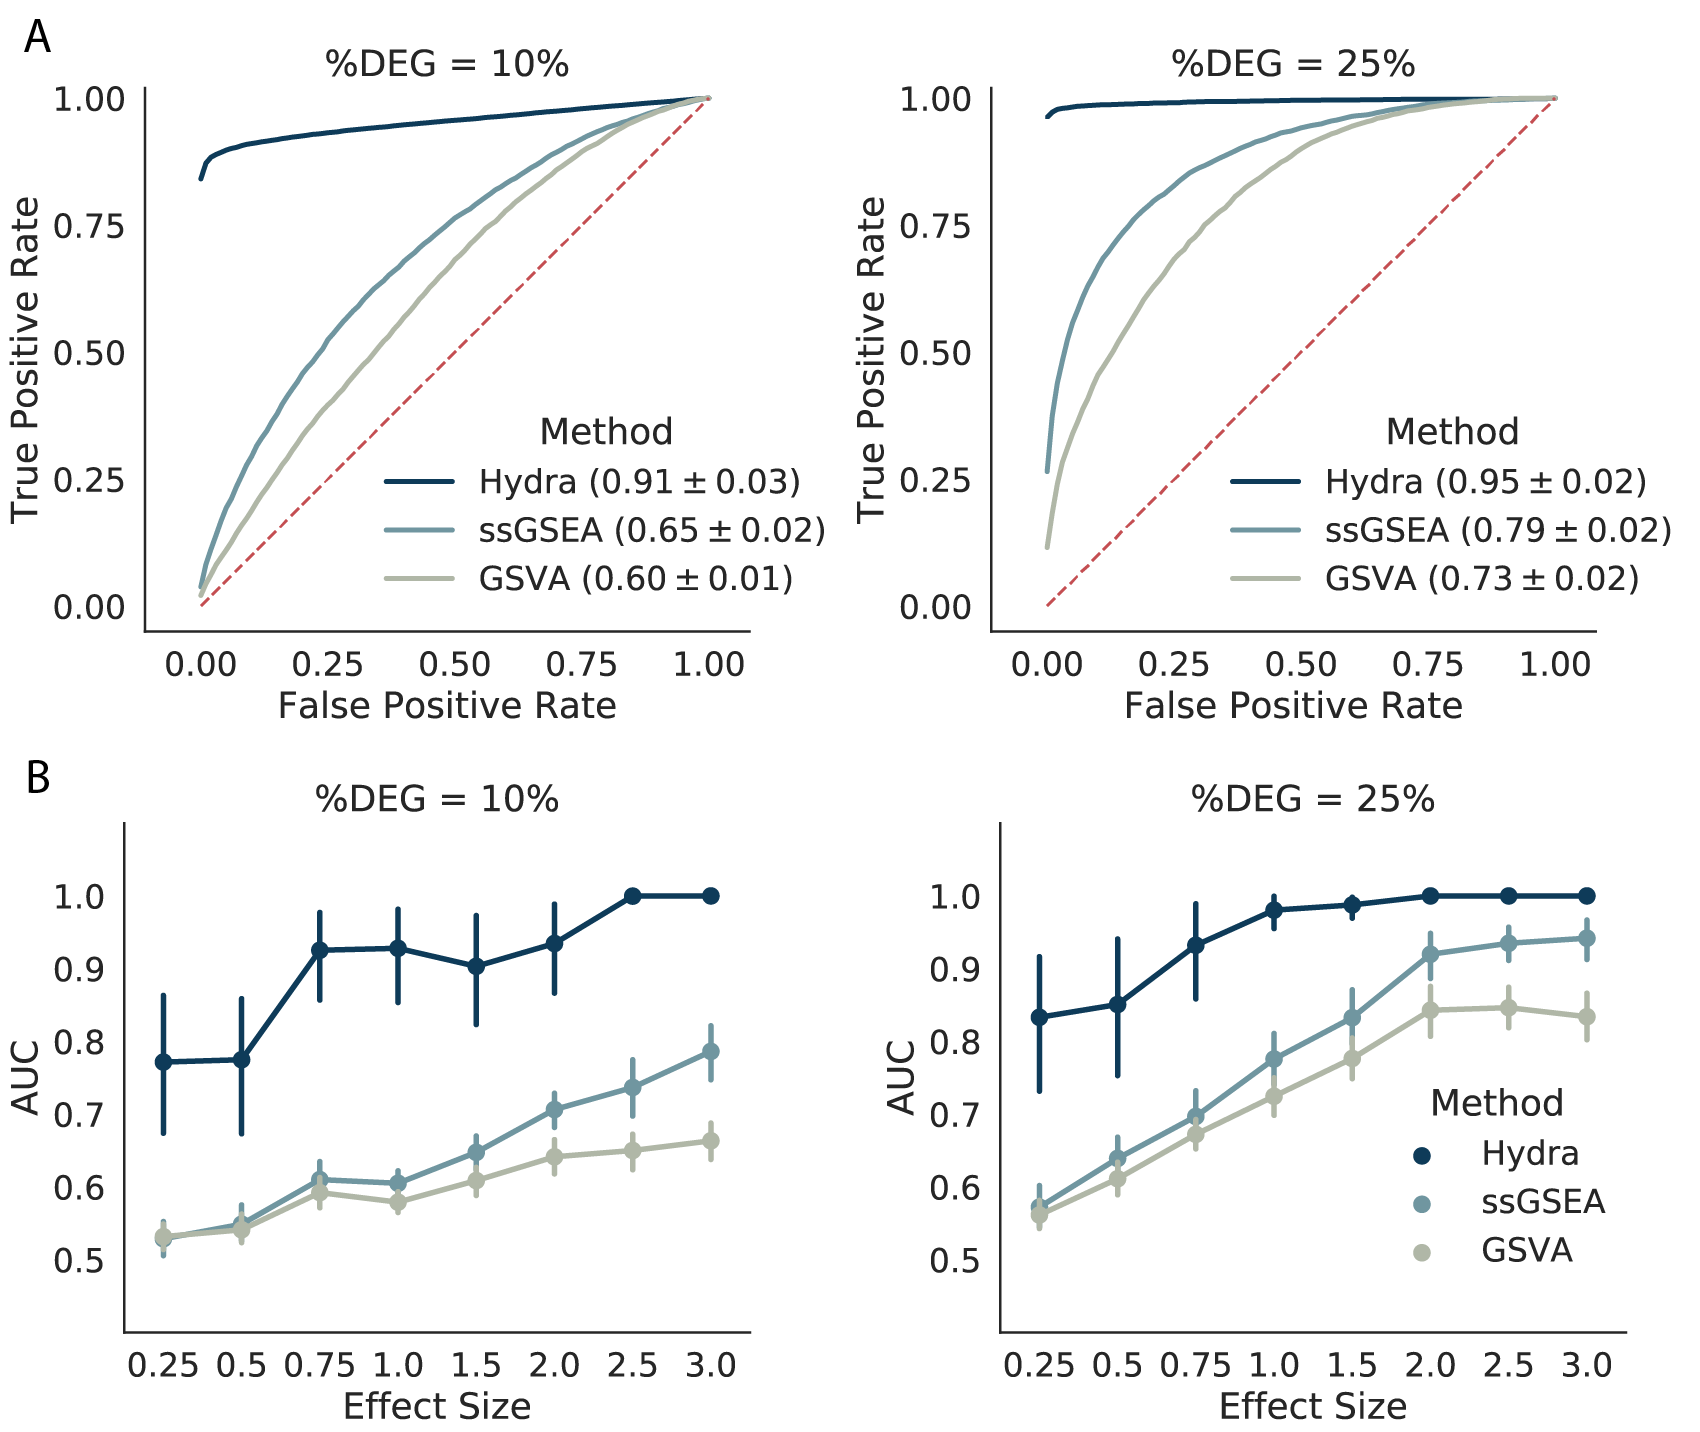
\includegraphics[width=\textwidth]{img/ROC-PLOT-2x}
	\caption{{\bf Hydra is more sensitive than available gene set enrichment approaches for detecting differential pathway expression in synthetic data.}
		(A) Mean receiver operator curves across effect sizes and MSigDB Hallmark gene sets. A larger area under the curve indicates better performance. (B) Line plots comparing the mean AUC at a range of effect sizes. (C) Scatter plots showing the relationship between area under the ROC curve (AUC), percent differentially expressed genes (\%DEG), effect size, and mean gene set expression.
		\label{rocplot}}
\end{figure}

We further investigated the performance of these methods by plotting the AUC against the effect size at \%DEG of 10 and 25\% (Fig. \ref{rocplot}B). The hydra method performed better across all effect sizes, achieving near perfect performance above an effect size of 1.0 and 0.75 at \%DEG of 10\% and 25\%, respectively. ssGSEA and GSVA performed similarly at low effect sizes, but ssGSEA performed better at \%DEG of 10\% and an effect size greater than 1.0. The performance difference between ssGSEA and GSVA was less pronounced at a higher \%DEG of 25\%. The ssGSEA and GSVA methods began to perform similarly to hydra at an effect size of 3.0 and \%DEG of 25\%. Therefore, the ranking approaches are less sensitive than the hydra approach, so the hydra approach is better suited for subtyping more homogeneous disease cohorts for precision medicine applications.

%TODO Check all figure references
\subsection{Hydra Analysis of High-Risk Neuroblastoma Identifies Distinct Tumor Microenvironment States}
After completing the performance assessment with synthetic gene expression data, we applied the hydra unsupervised enrichment analysis to the TARGET high-risk neuroblastoma cohort. High-risk neuroblastoma is an aggressive disease and is resistant to intensive therapy. Further subtyping of high-risk neuroblastoma may identify novel therapeutic targets and improve risk stratification. We hypothesized that unsupervised clustering of Gene Ontology terms would identify expression subtypes of high-risk neuroblastoma tumors. TumorMap analysis showed that the MYCN-non-amplified (MYCN-NA) neuroblastoma samples clustered separately from MYCN-amplified (MYCN-A) and stage 4S neuroblastomas (CITE) samples. We focused on the MYCN-NA neuroblastoma tumor samples because this is the largest set of samples (N=70), and variation within MYCN-NA tumors is not well understood \cite{morgensternChallengeDefiningUltrahighrisk2019a}.

\begin{figure}[!h]
	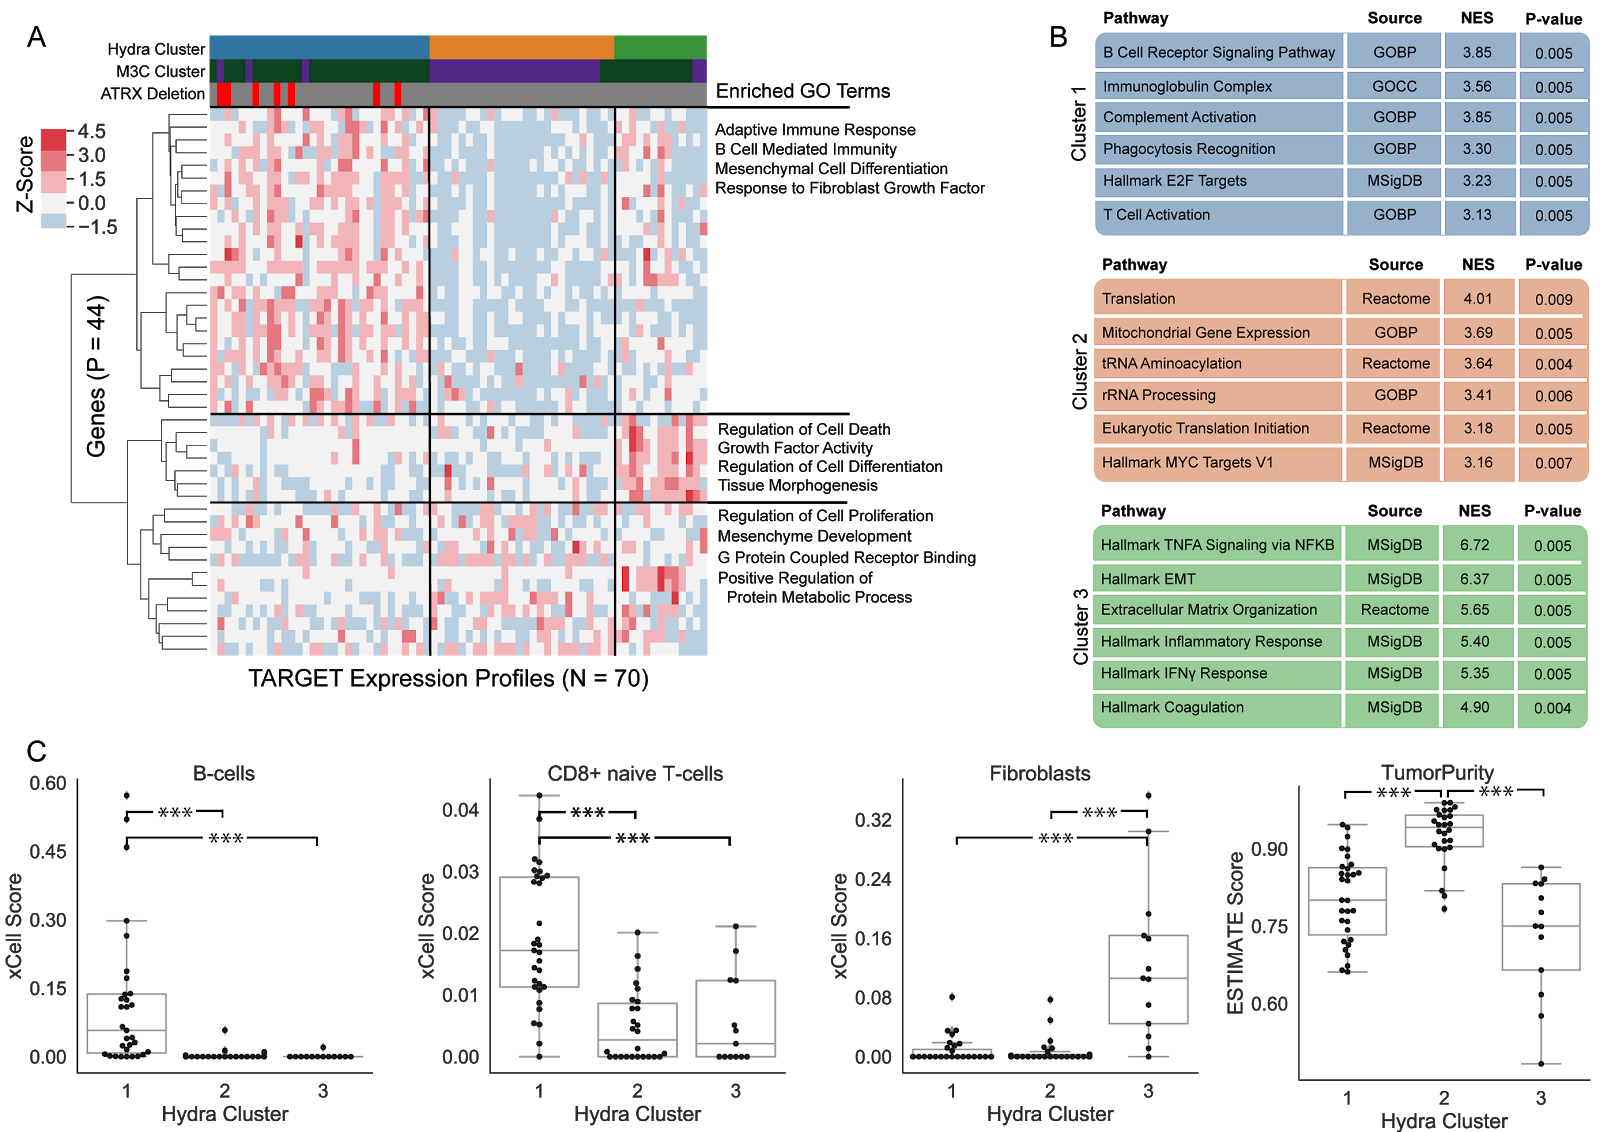
\includegraphics[width=\textwidth]{img/MYCN-NA-Figure-V5@2x}
	\caption{{\bf Hydra analysis identifies three distinct tumor microenvironment expression subtypes in MYCN non-amplified neuroblastoma samples.}
		A: Gene expression heatmap displaying expression profiles of hydra clusters. Heatmap columns (samples) are ordered by hydra cluster membership. Ward hierarchical clustering applied to rows (genes) identified coordinated expression of GO term genes. B: GSEA performed on each cluster identified enrichment of tumor microenvironment and proliferative signaling gene sets. C: xCell enrichment score distributions for B-cells, CD8+ naive T-cells, and Fibroblasts, and the ESTIMATE TumorPurity score distributions for each cluster; enrichments for all cell types are available in Supplemental Tables 3-5. Abbreviations: Normalized Enrichment Score (NES), Epithelial to Mesenchymal Transition (EMT), Gene Ontology Biological Process (GOBP).
		\label{MYCN-NA}}
\end{figure}

%TODO Fix supplementary table
We applied the hydra unsupervised enrichment analysis to the MYCN-NA cohort. The multimodal expression filter identified 428 genes with a minor component probability greater than 20\% (Supplementary Table 2). Gene Ontology analysis found enrichment for the following GO terms (FDR q < 0.01): adaptive immune response (24 genes), mesenchyme development (12 genes), steroid hormone secretion (4 genes), and response to corticosterone (4 genes). Multivariate Dirichlet process mixture model analysis of the 44 enriched GO term genes identified three clusters of neuroblastoma samples (Fig. \ref{MYCN-NA}A). The posterior probability for belonging to each cluster was 42\%, 34\%, and 17\%, respectively. The posterior probability for a sample belonging to a new cluster was about 6\% in our analysis. 

We next applied the cluster profiling gene set enrichment analysis (see Hydra Method section) to each cluster using all genes from the pre-filtered expression matrix. Cluster 1 was enriched for adaptive immune response gene sets, cluster 2 was enriched for proliferative signaling gene sets, and cluster 3 was enriched for cancer-associated fibroblast gene sets (Fig. \ref{MYCN-NA}B). Clusters 1 and 3 were enriched for tumor microenvironment-associated expression. To further validate this signal, we correlated the hydra clusters with enrichment scores from the tumor microenvironment profiling tools xCell \cite{aranXCellDigitallyPortraying2017} and ESTIMATE \cite{yoshiharaInferringTumourPurity2013a}. Cluster 1 had higher average xCell enrichment scores associated with adaptive immune cell types including B-cells, CD4+ naive T-cells, and CD8+ naive T-cells (Kruskal-Wallis: p $<$ 0.001; Supplementary Tables 3-5). Cluster 2 was characterized by the absence of immune and stromal expression and higher tumor purity. The average ESTIMATE tumor purity for each cluster was 88\%, 96\% and 82\%, respectively. Cluster 3 was enriched for fibroblast-associated expression by xCell analysis (Kruskal-Wallis: p $<$ 0.001). Clusters 1 and 3 had higher ESTIMATE immune-associated expression levels than cluster 2 (average ImmuneScore per cluster: 58, -612, 56), but cluster 3 had the highest stromal expression signature (average StromalScore per cluster: -1027, -1310, -135). We found no difference in patient survival outcomes across clusters (log-rank test, p $>$ 0.05). We investigated associations with clinical covariates, including mutation burden, age, and tumor content as assessed by a clinical pathologist, but found no statistically significant differences (Kruskal-Wallis: p $>$ 0.05; Supplementary Figure 2). We then investigated associations between the hydra clusters and neuroblastoma-associated molecular aberrations and clinical features (Supplementary Table 6). ATRX gene deletions were enriched in cluster 1 (Fisher’s Exact Test: p $<$ 0.05). MKI low tumors were enriched in cluster 2 and 3 (Fisher’s Exact Test: p $<$ 0.01). Chromosome 17 wild type tumors were enriched in clusters 2 and 3 (Fisher’s Exact Test: p $<$ 0.01).

Consensus clustering is a widely used approach for identifying tumor subtypes using gene expression data. We applied the M3C consensus clustering method, which is a more sophisticated version of consensus clustering that uses a null distribution to assess the statistical significance of the clustering \cite{johnM3CMonteCarlo2018, wilkersonConsensusClusterPlusClassDiscovery2010}.M3C clustering of the MYCN-NA expression data using the 5000 genes with the largest median absolute deviation (MAD) resulted in the identification of two statistically significant clusters. We found that the M3C clusters correlated with the hydra clusters with lower ESTIMATE TumorPurity, but were not able to separate the adaptive immune cell and fibroblast infiltrated clusters. We also applied kmeans clustering using the gap statistic approach for estimating the number of clusters, but this approach grouped all samples into a single cluster \cite{tibshirani2001estimating,maechler2012cluster}. We tested a range of gene variation thresholds, but found similar results across thresholds until the clustering became unstable at low gene numbers (\nameref{S3_Fig}). These results suggest the hydra approach is more sensitive at detecting distinct tumor microenvironment states.

\subsection{N-of-1 Tumor Analysis for Pediatric Neuroblastoma}
We investigated the predictive performance of the hydra approach for identifying clinically relevant signals in the N-of-1 tumor analysis setting. We obtained tumor gene expression data from five stage 4, MYCN-NA neuroblastoma samples (Fig. \ref{hefig}). The age at diagnosis ranged from 2 to 6 years. Four out of five samples had a deletion in the ATRX gene. Samples 1D and 1R are diagnosis and resection samples from the same patient. Three of the ATRX-deleted samples clustered with the high immune expression cluster (cluster 1) and one clustered in the low immune, high proliferative signaling cluster (cluster 2). Hydra analysis assigned sample 1D to cluster 1 and sample 1R to cluster 2. The resection sample 1R was extracted from lymph node tissue, which has a significantly different immune background than the training data. Another possible explanation for this change is that the tumor microenvironment is dynamic and the tumor may evade immune recognition as the disease progresses. We performed GSEA comparing samples 1D and 1R to investigate potential mechanisms leading to immune evasion in sample 1R. GSEA analysis found downregulation of the MHC Class I Antigen Processing \& Presentation GO term in sample 1R (adjusted p-value $<$ 0.002). Loss of antigen processing functions is a common mechanism of immune evasion across cancer types \cite{reevesAntigenProcessingImmune2017}.

\begin{figure}[!h]
	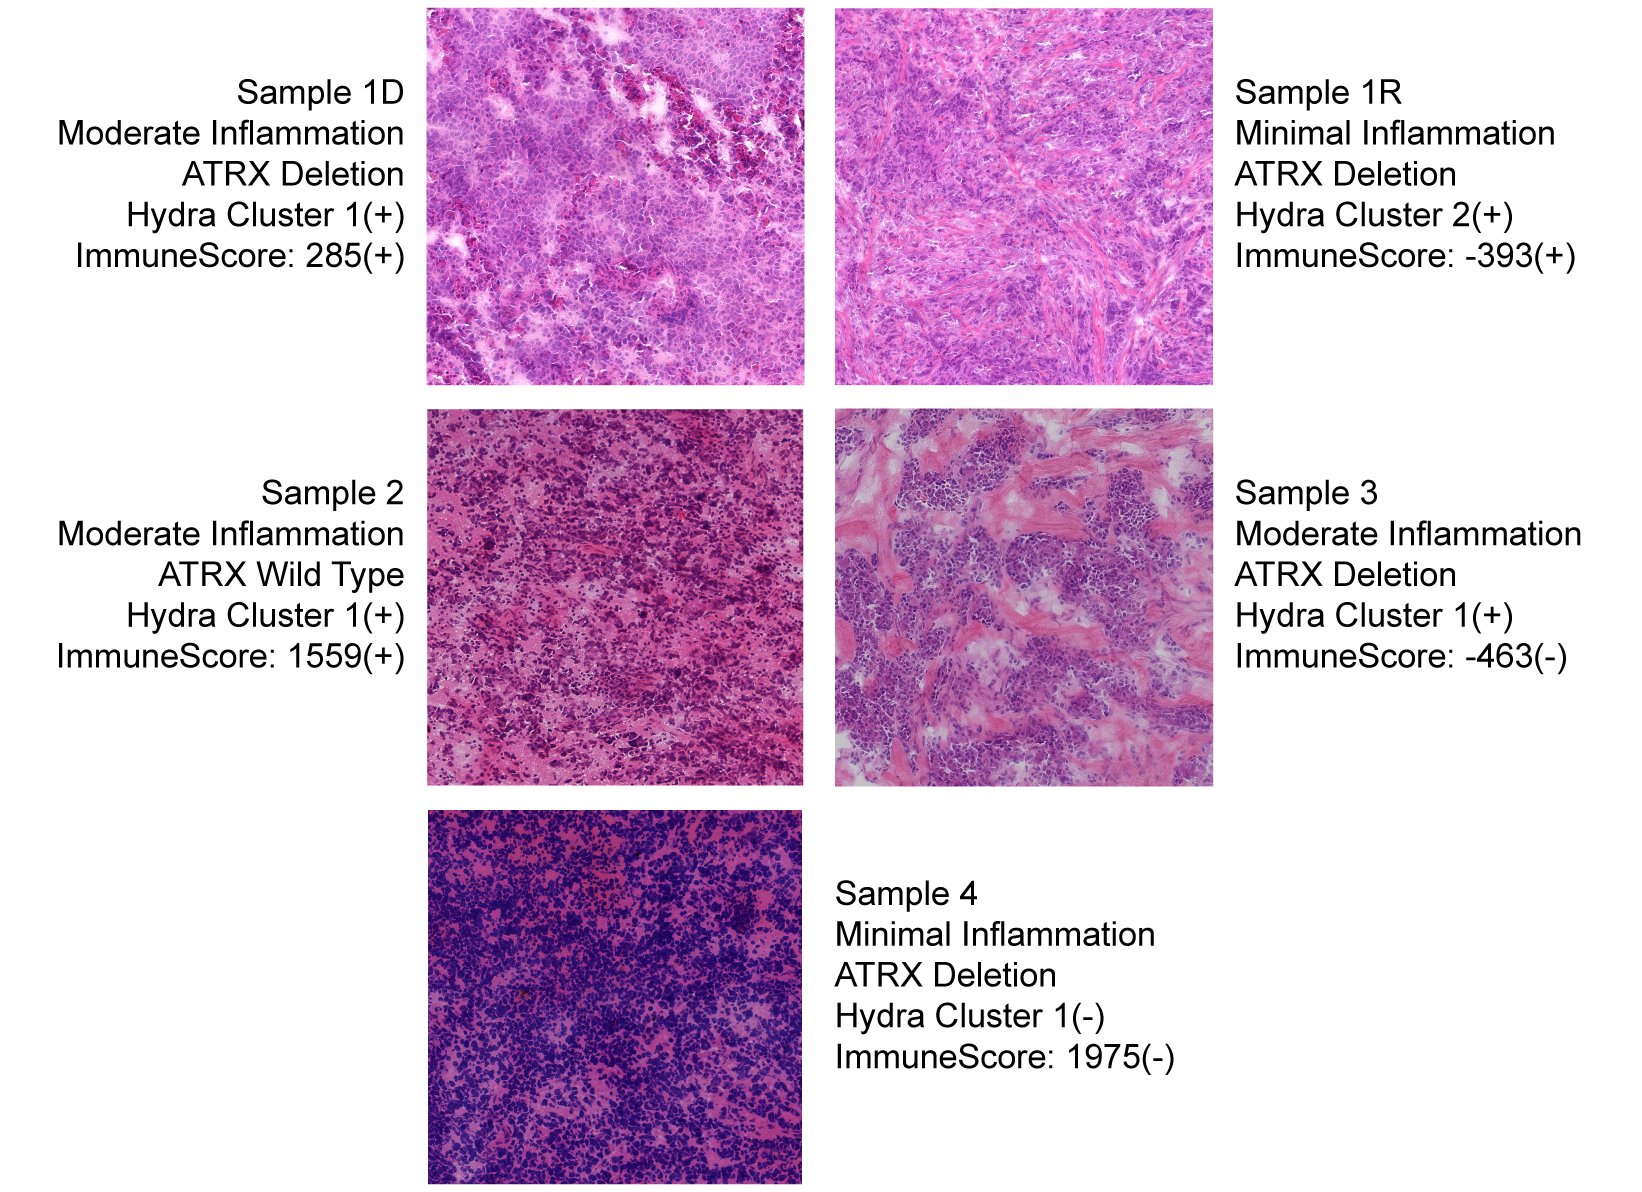
\includegraphics[width=\textwidth]{img/NBL-MYCN-NA-HE-2x}
	\caption{{\bf Hydra method correlates with histopathology review of tumor H\&E slides.}
		The tumor microenvironments of stage 4, MYCN-NA neuroblastoma patient samples were analyzed using gene expression and H\&E slide image data. Inflammation levels in the same tumor samples were assessed from H\&E slide images at 20x magnification (Moderate inflammation: 20-30\% lymphocyte content; Minimal inflammation: $<$ 10\% lymphocyte content). ATRX mutation status, hydra cluster assignment, and ESTIMATE ImmuneScore value are also indicated. Concordant and discordant predictions are marked with a positive (+) and negative (-) sign, respectively.}
	\label{hefig}
\end{figure}

We obtained H\&E slide images for these samples; the images were reviewed by a licensed pathologist and scored for evidence of inflammation. The N-of-1 predictive function of the hydra toolkit was used to classify samples into the subtypes discovered by the TARGET neuroblastoma analysis. Most of the samples (4 out of 5) clustered in cluster 1, which is characterized by higher immune marker expression. The hydra analysis agreed with the pathologist review in 4 out of 5 samples (Fig. \ref{hefig}). Sample 4 was the only discordant sample. Sample 4 is also from lymph node tissue, which may have higher immune expression because of the tissue type. Notably, concordant ESTIMATE values were present in 3 out of 5 samples scored by the pathologist: samples 1D, 1R, and 2. 

To further investigate expression patterns within the hydra-identified tumor microenvironment subtypes, we performed GSEA by z-score normalizing each tumor’s gene expression data to its tumor microenvironment cluster. This is a novel GSEA approach that uses the tumor microenvironment state discovered by the hydra approach to identify additional gene expression signals for individual samples. This approach revealed signals not present at the cohort level analysis (\nameref{S4_Fig}). For example, enrichment of immune expression signatures within cluster 2 predicted differences in overall survival such that patients with higher immune expression had a better overall survival rate. Similarly, an elevated cell cycle signal within cluster 3 predicted worse survival compared to other cluster 3 samples with lower cell cycle expression. This approach provides a more appropriate background distribution for determining the significance of gene expression patterns and survival statistics.

\subsection{Hydra Analysis Discovers Complex Tissue Signatures}
While the MYCN-NA neuroblastoma analysis focused on immune and fibroblast expression signatures, the hydra enrichment pipeline is unsupervised and is not restricted to immune or fibroblast signatures. For example, we applied the hydra enrichment analysis to the TARGET osteosarcoma cohort (N=74) and discovered enrichment of the GO striated muscle contraction term (FDR $<$ 0.01) \nameref{S5_Fig}. Multivariate clustering for the GO striated muscle contraction gene set using the sweep routine identified two clusters. xCell analysis of the osteosarcoma cohort found significant enrichment of skeletal muscle expression in the second cluster (Mann-Whitney U test, p $<$ 0.001). Surprisingly, the M3C clustering approach was not able to detect the strong muscle signature using the 5000 genes with the largest MAD (p $>$ 0.05). We identified a similar expression signal in an independent cohort of osteosarcoma tumor samples and subsequently confirmed with a licensed pathologist that the tumor sample did in fact contain muscle tissue. Explaining these sources of variation is necessary to derive clinically relevant conclusions from gene expression data. 

Similarly, over-expression analysis of Ewing sarcoma identified JAK1 as a potential druggable gene, but analysis of the multimodal expression of the JAK1 gene revealed that over-expression of JAK1 may be related to higher infiltration of MAST cells (\nameref{S6_Fig}. Inhibitors of JAK1 were shown to inhibit MAST cell functions, which could be an unintended consequence of a targeted therapy approach \cite{hermansJAK1JAK2Inhibitor2018}. Therefore, the hydra approach reveals important gene expression signatures reflecting cell content within the tumor sample and is widely applicable for revealing important gene expression signatures in complex tumor samples.

\subsection{Hydra Analysis Reveals Related Expression Subtypes Across Pediatric Cancers}
We next wanted to see if similar hydra clusters could be identified across small round blue cell tumors. We first performed TumorMap analysis which is a dimensionality reduction approach for visualizing genomic data on a 2D plane \cite{newtonTumorMapExploringMolecular2017}. We found that MYCN-NA neuroblastoma, osteosarcoma, Ewing sarcoma, synovial sarcoma, alveolar rhabdomyosarcoma, and embyronal rhabdomyosarcoma all form distinct clusters (Fig. \ref{pancan}). This suggests there is a strong cell of origin signal that yields separable expression profiles. This is an observation that was recently made in the larger TCGA data set \cite{Hoadley2014}. We next performed hydra analysis within each cancer type and found similar biological themes in the disease-specific GSEA cluster profiling analysis. We next performed hierarchical clustering for the top 10 statistically significant gene sets for each disease and found that this led to the diseases clustering by their hydra cluster gene set enrichment (Fig. \ref{pancan}). Common themes emerged across diseases including translational regulation, cell cycle regulation, immune effector cell signals, inflammation, extracellular matrix organization, and tissue-of-origin signals. Furthermore, we found that these signals predicted differences in patient outcomes in osteosarcoma and synovial sarcoma, two diseases for which we had patient outcome data. In both cases, the presence of immune associated expression correlated with better patient outcomes compared to tumors with proliferative signaling pathways associated with the upregulation of translation initiation.


\begin{figure}[!h]
	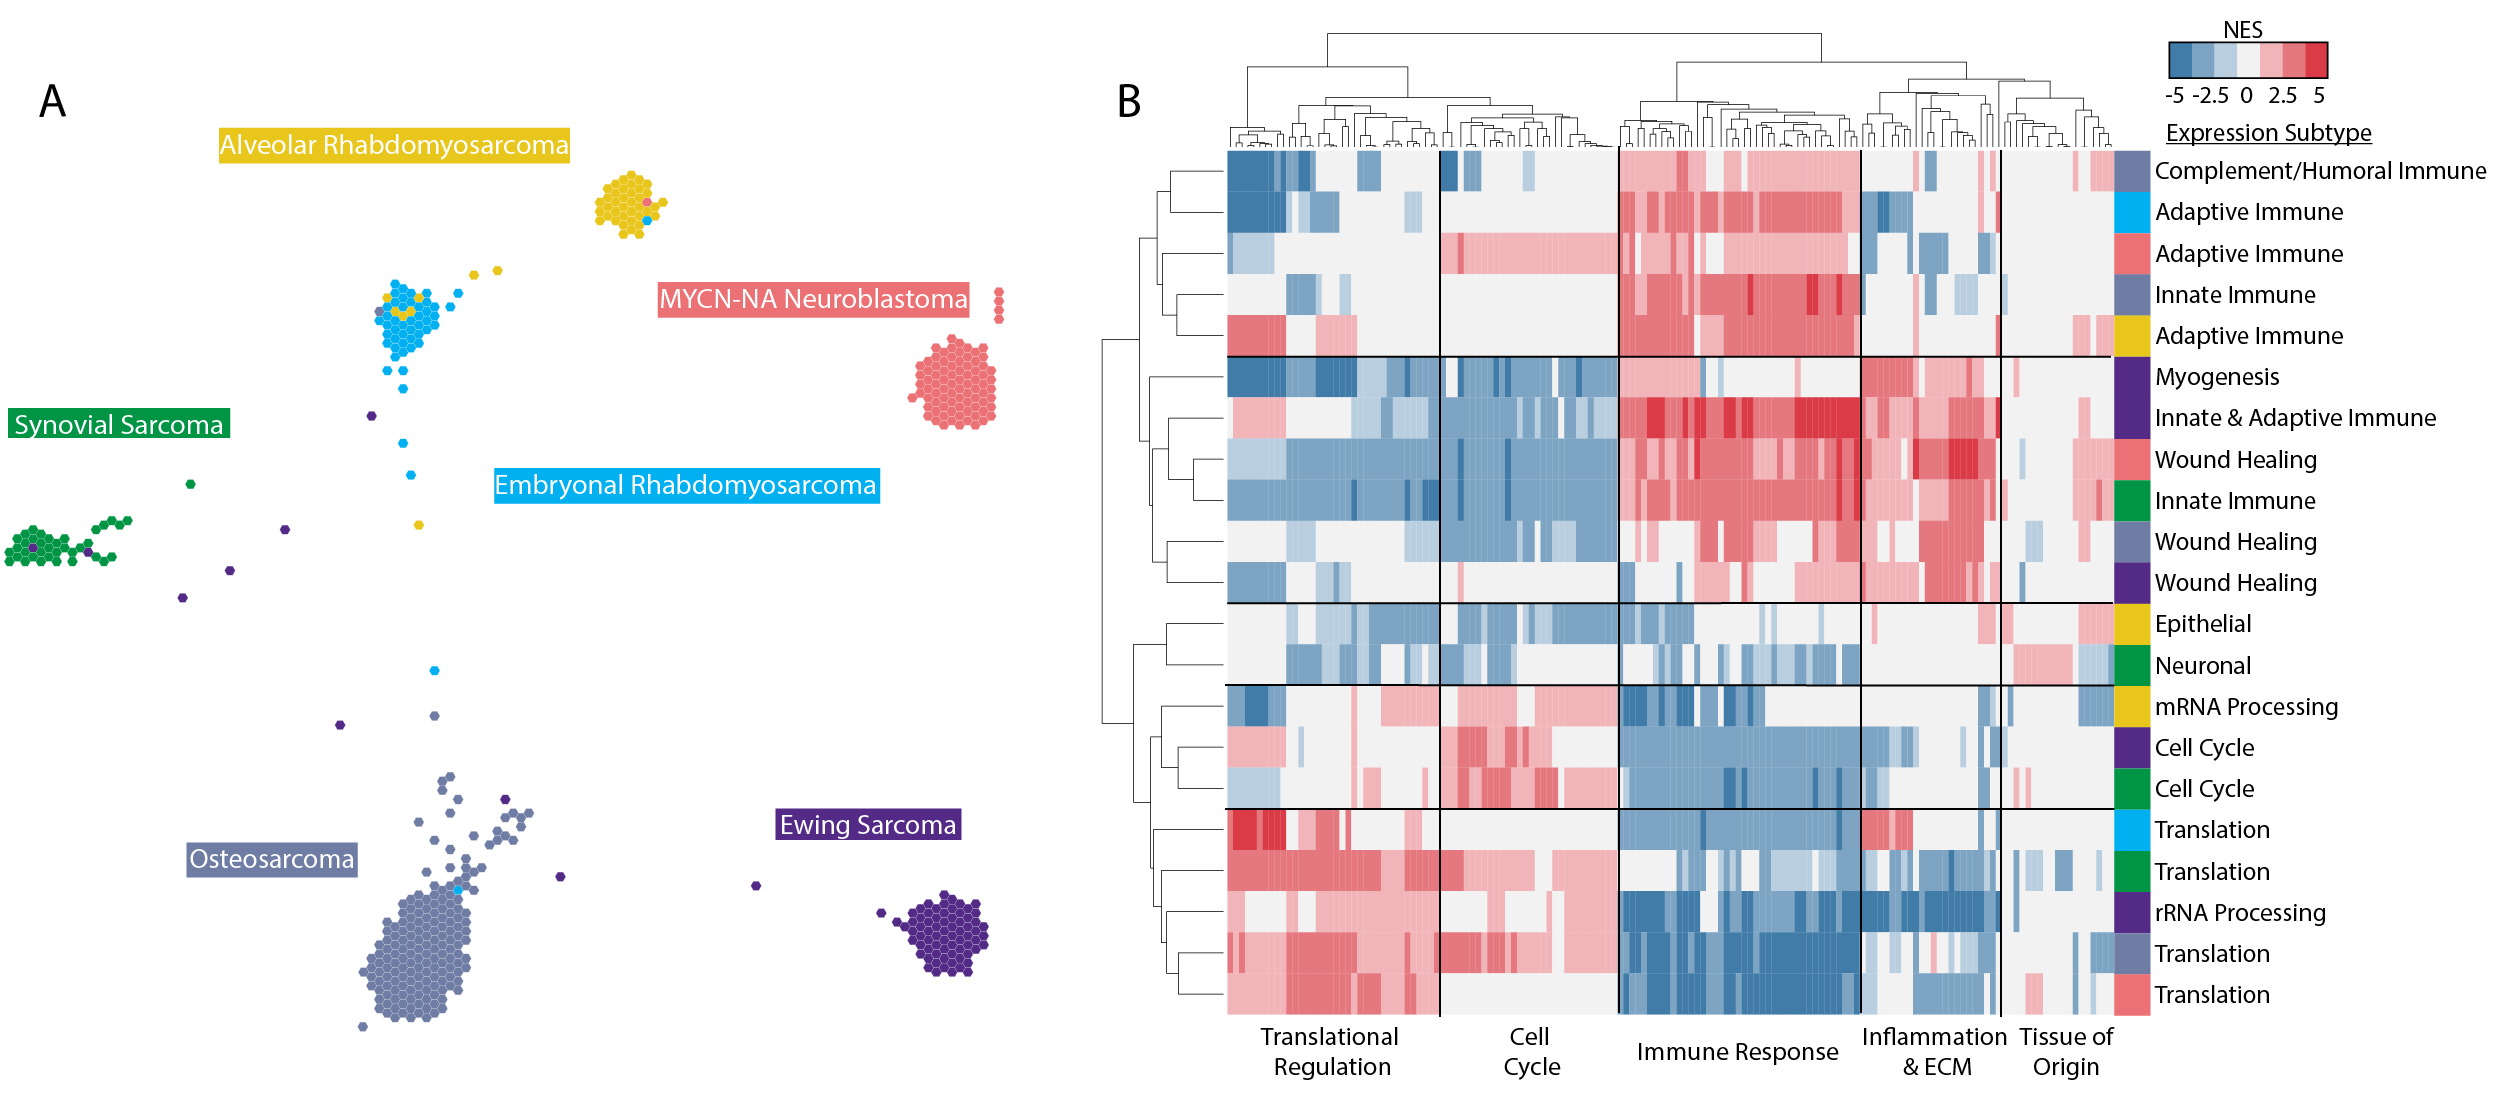
\includegraphics[width=1.05\textwidth]{img/hydra-pan-small-round-blue-V2-2x}
	\caption{{\bf Hydra analysis of small round blue cell tumors reveals similar expression subtypes across cancer types.} A: TumorMap visualization of 6 different small round blue cell tumor types. B: Hierarchically clustered heatmap of gene set normalized enrichment scores (NES) for the top 10 enriched gene sets for each disease type. The cancer type color bar corresponds to the cancer type color in panel A. The expression subtype was manually assigned after reviewing the most highly enriched gene sets for each hydra cluster.}
	\label{pancan}
\end{figure}


\section*{Discussion}
The hydra framework uses model-based clustering to identify recurrent expression patterns within cancer gene expression cohorts. We leveraged recent improvements in model-based clustering algorithms to identify differentially expressed genes without a matched normal distribution. We modeled differential expression as a multimodal Gaussian distribution using nonparametric Bayesian statistics. We then enriched for biologically-annotated Gene Ontology terms and performed multivariate clustering to reveal cancer subtyping expression signatures. The hydra framework can be used for identifying expression subtypes and classifying N-of-1 tumors. The hydra framework outperformed standard gene set enrichment tools for identifying overexpression of the MSigDB Hallmark cancer gene sets in synthetic cancer gene expression data and identified tumor microenvironment gene expression signatures in the TARGET pediatric neuroblastoma and osteosarcoma datasets that were not detected by consensus clustering analysis. 

Multivariate gene expression analysis is typically underpowered because the number of genes greatly exceeds the number of samples. To address this limitation, we propose selecting for multimodally expressed genes before performing multivariate analysis. The hydra multimodal filter reduces the number of genes and enriches for genes that participate in known biological processes, including those curated in the Gene Ontology database. As Yi Li et al. (2005) found in their study on unsupervised clustering of gene expression data, we also found that reducing expression data to multimodally expressed genes improves clustering of clinical subtypes in pediatric cancers. For example, multimodally expressed genes separate neuroblastoma subtypes by TumorMap analysis better than the standard approach of using all expressed genes. Furthermore, we showed that the hydra approach is more sensitive at resolving tumor microenvironment subtypes than the M3C consensus clustering approach.

Significant progress has been made in subtyping neuroblastomas and adapting therapy for aggressive subtypes, but unexplained heterogeneity remains. Not accounting for this heterogeneity decreases the power of standard methods to detect important expression patterns. Identifying biomarkers using genome-wide technology may lead to improved risk stratification and the discovery of novel drug targets \cite{morgensternChallengeDefiningUltrahighrisk2019a}. Hydra analysis of the TARGET MYCN-NA neuroblastoma cohort (N=70) found differential expression of tumor microenvironment markers, including markers of the adaptive immune response. Pediatric cancers are generally thought to be non-immunogenic because they have lower mutation burden than adult cancers, but the immunogenicity of pediatric cancer has not been sufficiently investigated \cite{majzner2017harnessing}. Our analysis found significant variation in immune marker expression and identified ATRX deletions as a potential biomarker of immune infiltrated tumors. Further investigation into gene expression signatures and molecular aberrations that predict response to immunotherapy in pediatric cancers is needed. Hydra analysis may facilitate the development of novel therapies by grouping patients with similar tumor microenvironment properties.

We found significant differences in immune and stromal expression that may inform precision medicine applications. The tumor microenvironment has become an important therapeutic consideration, but few methods account for the tumor microenvironment directly. Tumor purity has been identified as a confounding factor in cancer gene expression subtyping efforts \cite{rheeImpactTumorPurity2018}. For example, tumor purity and tumor microenvironment expression have been shown to correlate with pancreatic cancer subtypes \cite{raphael2017integrated}. Furthermore, Aran et al. (2018) found that tumor purity was correlated with the mesenchymal glioblastoma subtype and recommended a differential expression approach to computationally remove the tumor purity signal. However, standard approaches for subtracting the tumor purity effect may not be the best approach because several mechanisms may influence tumor purity, and each mechanism may result in a different expression pattern. For instance, our analysis of MYCN-NA neuroblastoma identified two gene expression signatures that correlated with lower predicted tumor purity. Cluster 1 had an adaptive immune expression signature and cluster 3 had a cancer-associated fibroblast signature. Therefore, the estimated tumor purity signal should not be subtracted without first accounting for the different mechanisms influencing tumor purity.

\section*{Conclusion}
Precision oncology aims to differentiate tumors of the same diagnosis in order to match patients with the best treatment. We have developed the hydra method to discover subtle but recurrent expression patterns within a cancer type. Our approach may help to uncover the biology underlying tumor progression and response to therapy. We have shown that hydra is more sensitive than standard gene set enrichment approaches for detecting differential pathway expression. Additionally, we applied the unsupervised hydra analysis to pediatric neuroblastoma and osteosarcoma data and discovered distinct tumor microenvironment states. The hydra pipeline is a sensitive unsupervised clustering approach for N-of-1 tumor analysis and will facilitate pediatric precision oncology by discovering expression subtype signatures.

\section*{Supporting information}

% Include only the SI item label in the paragraph heading. Use the \nameref{label} command to cite SI items in the text.
\paragraph*{S1 Fig.}
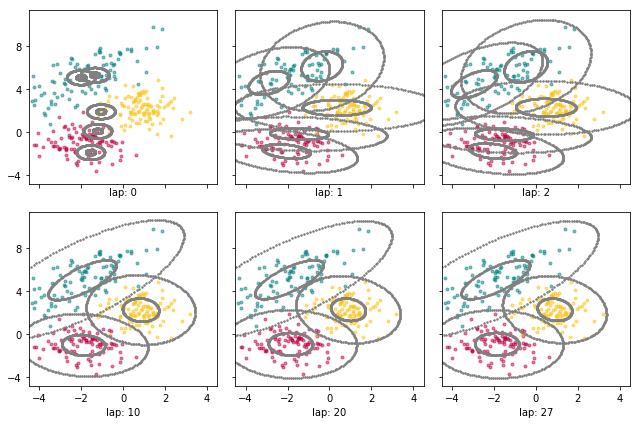
\includegraphics[width=\textwidth]{img/bnpy-example-fit}
\label{S1_Fig}
{\bf Example of iterative model fit process on synthetic data.} We used the bnpy moVB algorithm to infer the number of clusters from the data. The model first randomly assigns clusters to the data and iteratively improves the model fit, creating and destroying clusters until the model converges on the correct number of clusters \cite{hughesBnpyReliableScalable}. 

\paragraph*{S2 Fig.}
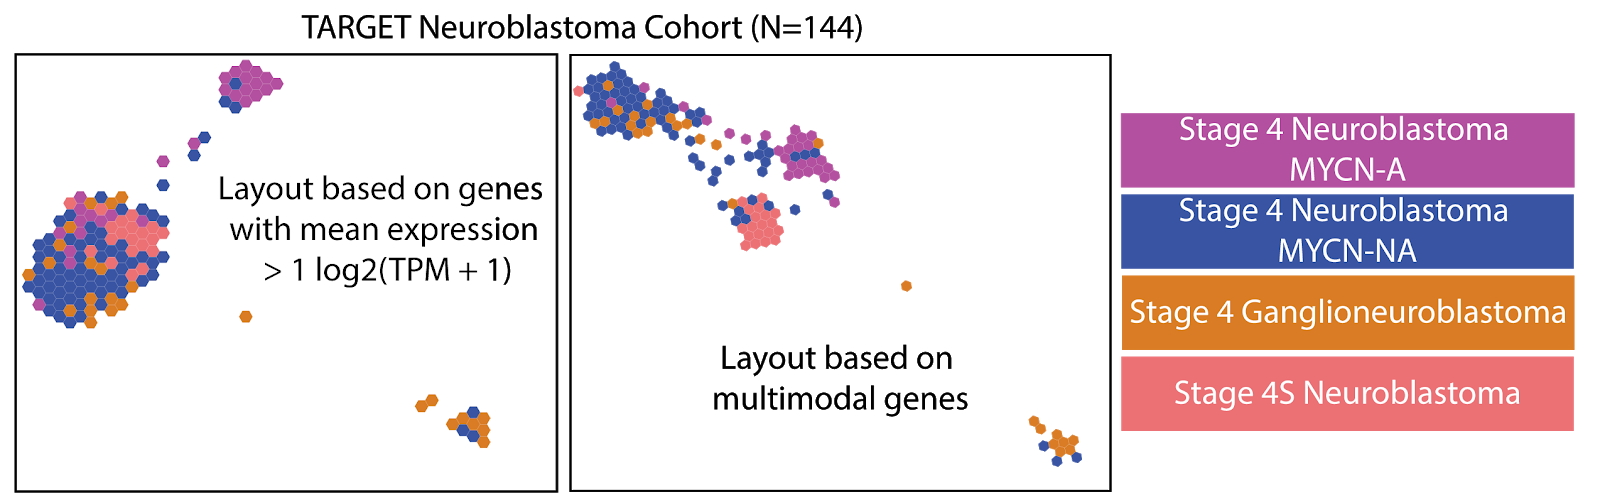
\includegraphics[width=\textwidth]{img/TumorMap-NBL-MM-V3-2x}
\label{S2_Fig}
{\bf Enriching for multimodally expressed genes improves clustering of established neuroblastoma subtypes.} Standard TumorMap analysis (Newton et al. 2017) of the TARGET neuroblastoma dataset resulted in stage 4S samples clustering with stage 4 neuroblastoma samples (left). An alternative TumorMap based solely on 1,498 multimodally expressed genes separated the stage 4S samples into a distinct cluster (right).

\paragraph*{S3 Fig.}
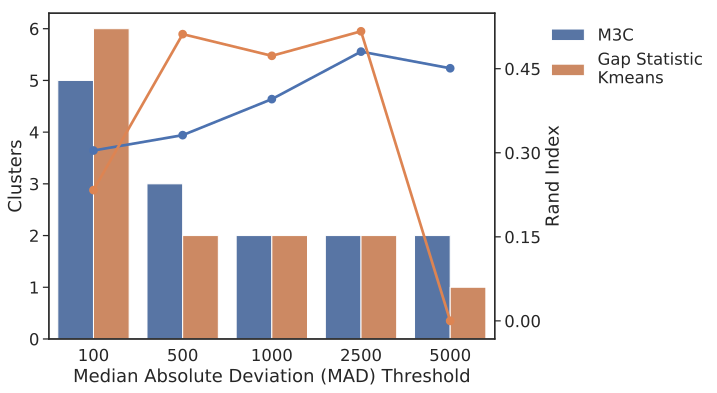
\includegraphics[width=0.75\textwidth]{img/clustering-screen}
\label{S3_Fig}
{\bf{Consensus and Gap statistic k-means clustering applied to TARGET MYCN-NA cohort.}} We tested a range of gene expression variation thresholds based on the median absolute deviation, but found that the clusters identified by this approach could not resolve the same clusters as the hydra approach. The barplot visualized the number of clusters and the lineplot tracks the Rand index for those clusters and the hydra clusters.

\paragraph*{S4 Fig.}
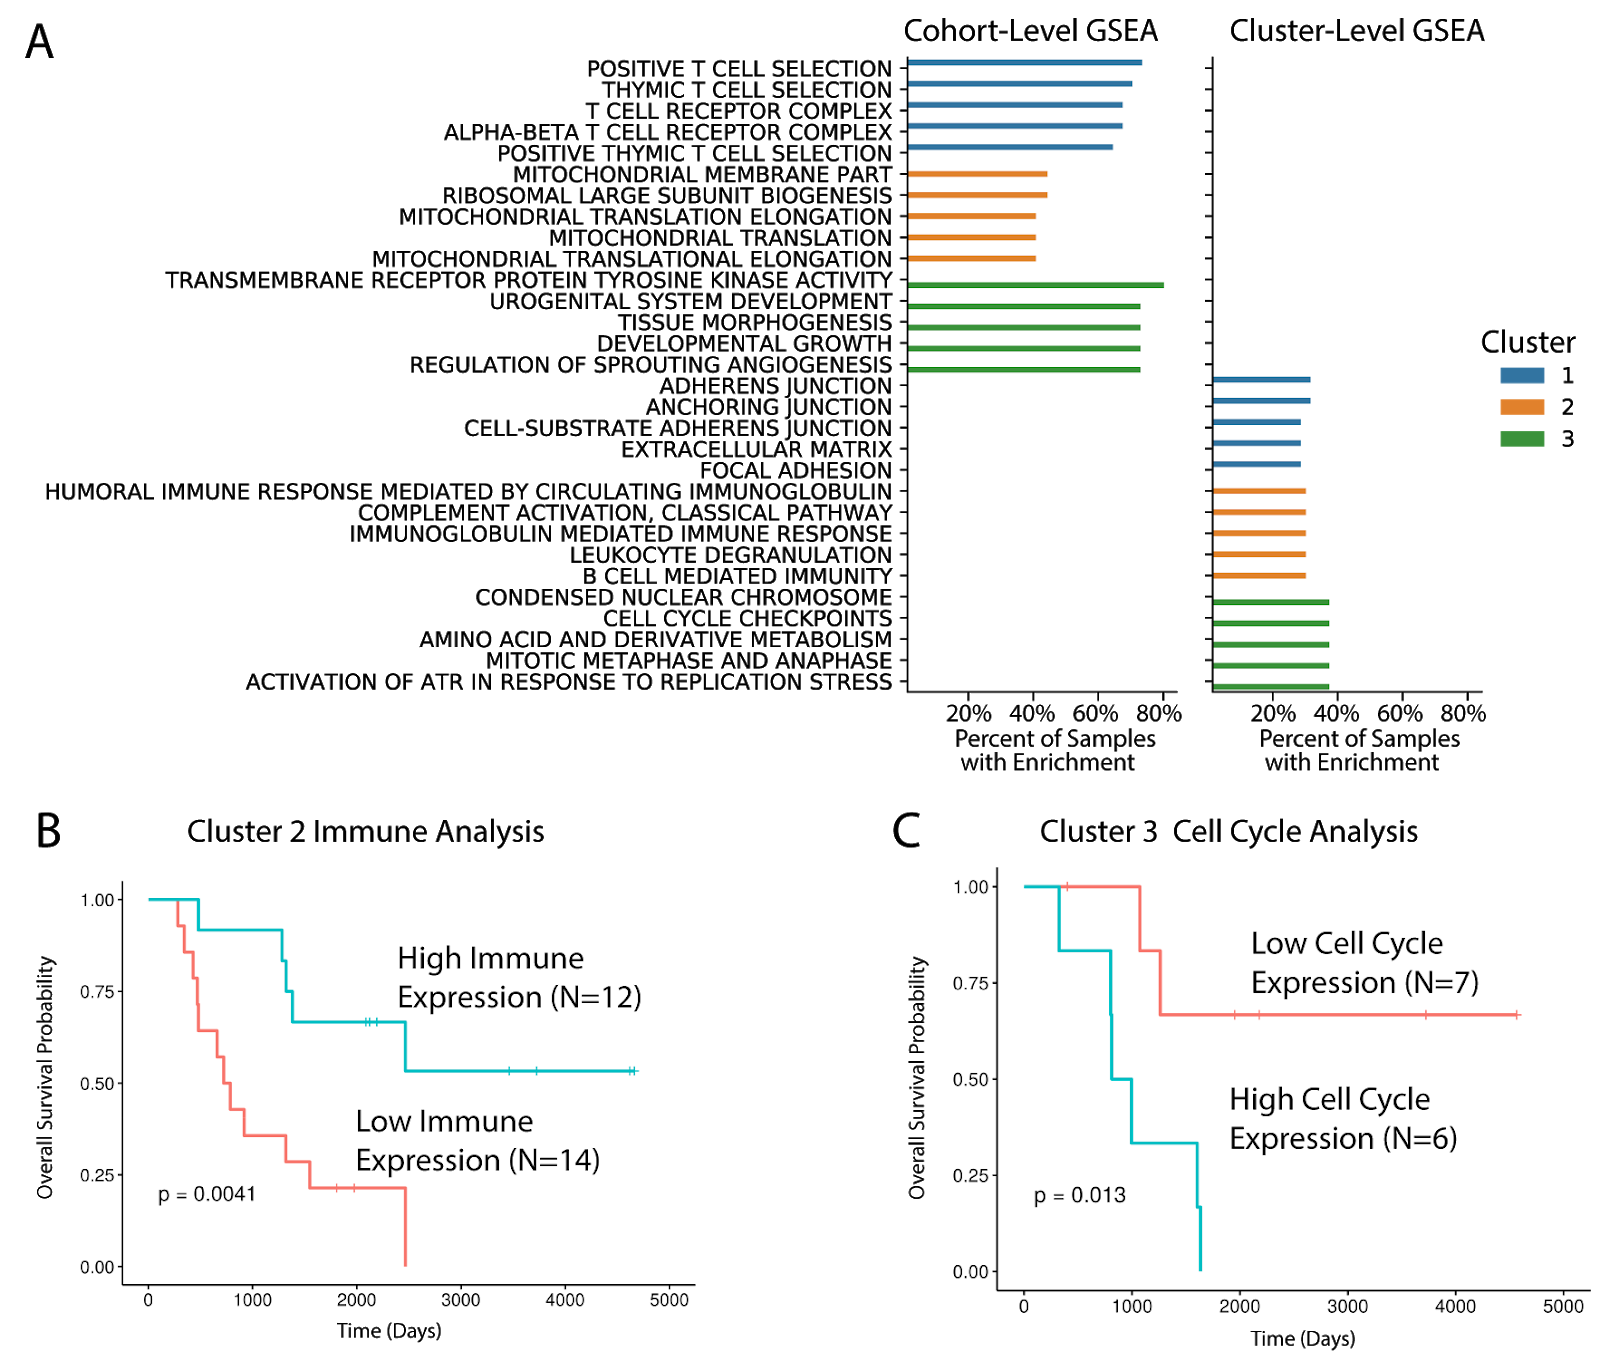
\includegraphics[width=\textwidth]{img/SubCluster-Analysis-V2@2x.png}
\label{S4_Fig} {\bf Gene set enrichment analysis (GSEA) of MYCN-NA neuroblastoma identifies survival differences within hydra cluster 2 and cluster 3.} (A) Top 5 differentially enriched gene sets for each cluster comparing the entire MYCN-NA neuroblastoma cohort (cohort-level GSEA) and the corresponding hydra cluster (cluster-level GSEA). GSEA analysis of the hydra clusters found immune and cell cycle signals that were not identified in the cohort-level analysis. (B \& C) GSEA separated cluster 2 into high and low immune subtypes and cluster 3 into high and low cell cycle subtypes. These signals correlated with differences in overall survival. 

\paragraph*{S5 Fig.}
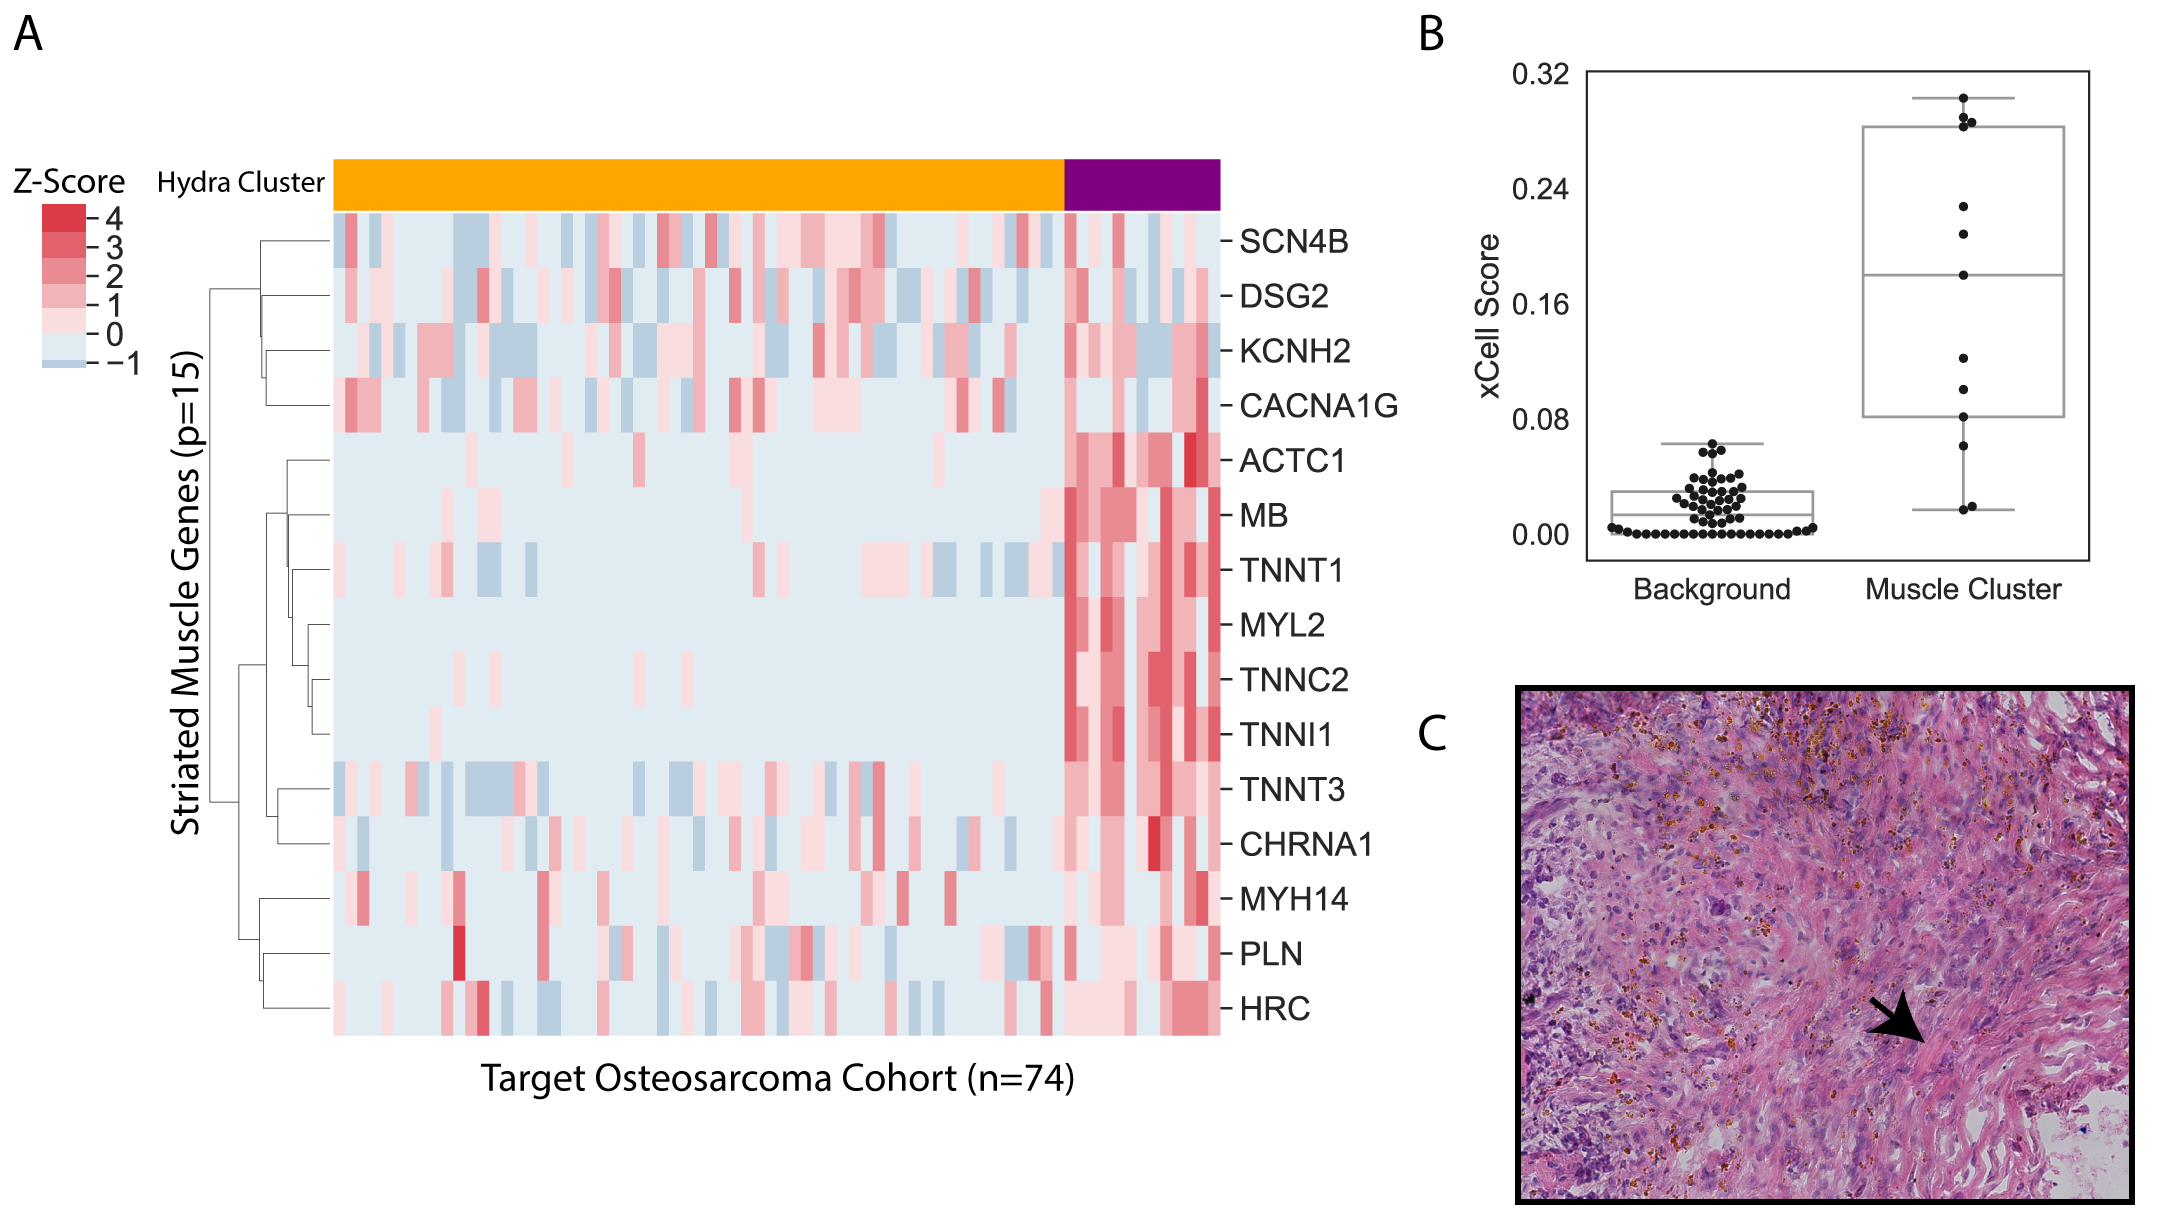
\includegraphics[width=\textwidth]{img/muscle-signature-genes-2x}
\label{S5_Fig} {\bf Hydra analysis of TARGET osteosarcoma cohort reveals skeletal muscle signature.} Hydra enrichment analysis on the TARGET osteosarcoma cohort revealed a subset of patients with high skeletal muscle expression. (A) Clustered heatmap shows the muscle signature genes identified by hydra unsupervised enrichment analysis. (B) xCell tumor microenvironment profiling identified significant differences in skeletal muscle expression compared to background (p < 0.001). (C) H\&E stained tumor slide for an independent osteosarcoma sample confirms presence of striated muscle tissue within the sequenced tumor sample.

% Add panel labels
\paragraph*{S6 Fig.}
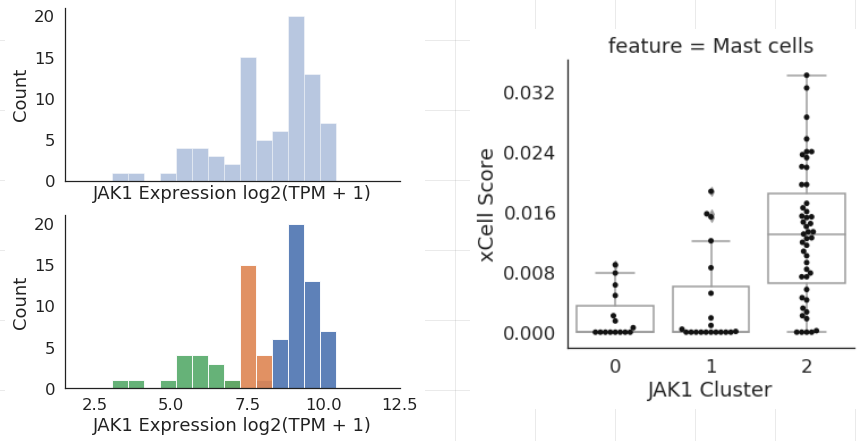
\includegraphics[width=\textwidth]{img/Selection_026}
\label{S6_Fig} {\bf Hydra analysis identifies expression of druggable JAK1 gene in Ewing sarcoma correlates with infiltrating mast cell expression.} Here we show the utility of the mixture model approach for identifying important gene expression patterns for precision medicine applications. JAK1 is a druggable gene, but is also an important gene in immune cell signaling pathways. We found that expression of JAK1 in Ewing sarcoma correlated with the mast cell expression. Interestingly, the JAK1 inhibitor ruxolitinib was shown to inhibit mast cell functions \cite{hermansJAK1JAK2Inhibitor2018}, accounting for the tumor microenvironment expression is an important step in developing precision medicine approaches for pediatric cancers.

\begin{table}
	\label{S1_Table}
	\caption*{\bf{S1 Table}}
	\subcaption{Osteosarcoma Translational Regulation Cluster}
	\begin{tabular}{L{10cm}R{1.5cm}R{1.5cm}}
		\toprule
		Pathway &      Adjusted P-value &   NES \\
		\midrule
		TRANSLATION (REACTOME) &  1.56e-03 &  4.14 \\
		CHROMOSOME MAINTENANCE (REACTOME) &  1.52e-03 &  3.95 \\
		MITOCHONDRIAL TRANSLATIONAL ELONGATION (GOBP) &  1.52e-03 &  3.84 \\
		HALLMARK\_E2F\_TARGETS (MSIGDB\_C2) &  1.52e-03 &  3.84 \\
		TRANSLATION (GOBP) &  1.57e-03 &  3.83 \\
		MITOCHONDRIAL TRANSLATION ELONGATION (REACTOME) &  1.52e-03 &  3.82 \\
		HALLMARK\_MYC\_TARGETS\_V1 (MSIGDB\_C2) &  1.52e-03 &  3.80 \\
		DEPOSITION OF NEW CENPA-CONTAINING NUCLEOSOMES (REACTOME) &  1.52e-03 &  3.78 \\
		NUCLEOSOME ASSEMBLY (REACTOME) &  1.52e-03 &  3.78 \\
		MITOCHONDRIAL TRANSLATION TERMINATION (REACTOME) &  1.52e-03 &  3.75 \\
		\bottomrule
	\end{tabular}
	
	\bigskip

	\subcaption{Osteosarcoma Wound Healing Cluster}
	\begin{tabular}{L{10cm}R{1.5cm}R{1.5cm}}
		\toprule
		Pathway &  Adjusted P-value &   NES \\
		\midrule
		EXTRACELLULAR MATRIX ORGANIZATION (GOBP) &  0.04 &  4.38 \\
		EXTRACELLULAR STRUCTURE ORGANIZATION (GOBP) &  0.05 &  4.38 \\
		NABA\_CORE\_MATRISOME (MSIGDB\_C2) &  0.04 &  4.02 \\
		HALLMARK\_INFLAMMATORY\_RESPONSE (MSIGDB\_C2) &  0.03 &  3.97 \\
		TYROBP CAUSAL NETWORK (WIKIPATHWAYS\_20181110) &  0.01 &  3.93 \\
		PID\_AVB3\_INTEGRIN\_PATHWAY (MSIGDB\_C2) &  0.02 &  3.91 \\
		HALLMARK\_COAGULATION (MSIGDB\_C2) &  0.02 &  3.90 \\
		HALLMARK\_EPITHELIAL\_MESENCHYMAL\_TRANSITION (MSIGDB\_C2) &  0.04 &  3.89 \\
		PID\_INTEGRIN1\_PATHWAY (MSIGDB\_C2) &  0.01 &  3.88 \\
		BETA1 INTEGRIN CELL SURFACE INTERACTIONS (PID) &  0.01 &  3.88 \\
		\bottomrule
	\end{tabular}
	
	\ContinuedFloat
	
	\subcaption{Osteosarcoma Overall Survival}
	\centering
	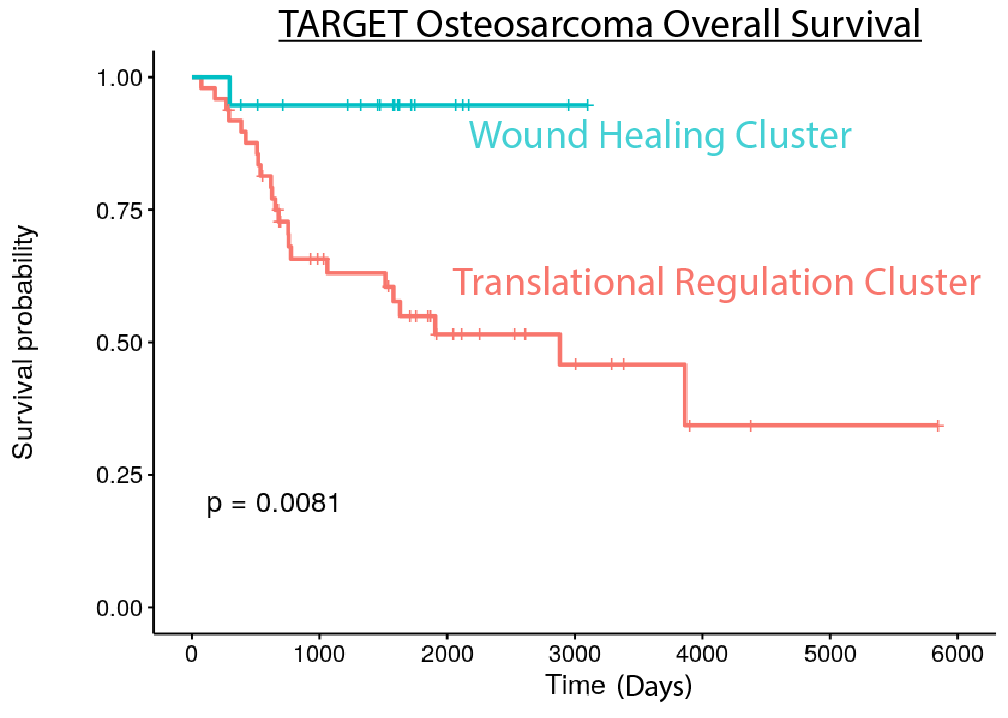
\includegraphics[width=0.75\textwidth]{img/osteo-kaplan-meier-2x}	
\end{table}

\FloatBarrier

\begin{table}
	\label{S2_Table}
	\caption*{\bf{S2 Table}}
	\subcaption{Synovial Sarcoma Translational Regulation Cluster}
	\begin{tabular}{L{10cm}R{1.5cm}R{1.5cm}}
		\toprule
		Pathway &      Adjusted P-Value &   NES \\
		\midrule
		TRANSLATION (REACTOME) &  3.36e-03 &  4.52 \\
		TRANSLATION (GOBP) &  3.36e-03 &  4.42 \\
		RIBOSOME BIOGENESIS (GOBP) &  3.36e-03 &  4.42 \\
		RNA PROCESSING (REACTOME) &  3.36e-03 &  4.29 \\
		RRNA PROCESSING IN THE NUCLEUS AND CYTOSOL (REACTOME) &  3.36e-03 &  4.25 \\
		MAJOR PATHWAY OF RRNA PROCESSING (REACTOME) &  3.36e-03 &  4.22 \\
		PEPTIDE BIOSYNTHETIC PROCESS (GOBP) &  3.36e-03 &  4.17 \\
		RRNA PROCESSING (GOBP) &  3.36e-03 &  4.16 \\
		NCRNA PROCESSING (GOBP) &  3.36e-03 &  4.16 \\
		HALLMARK\_MYC\_TARGETS\_V1 (MSIGDB\_C2) &  3.36e-03 &  4.09 \\
		\bottomrule
	\end{tabular}
	
	\bigskip
	\ContinuedFloat
	
	\subcaption{Synovial Sarcoma Innate Immune Cluster}
	\begin{tabular}{L{10cm}R{1.5cm}R{1.5cm}}
		\toprule
		Pathway &      Adjusted P-value &   NES \\
		\midrule
		HALLMARK\_INTERFERON\_GAMMA\_RESPONSE (MSIGDB\_C2) &  1.77e-03 &  5.11 \\
		HALLMARK\_INFLAMMATORY\_RESPONSE (MSIGDB\_C2) &  1.77e-03 &  5.01 \\
		HALLMARK\_TNFA\_SIGNALING\_VIA\_NFKB (MSIGDB\_C2) &  1.77e-03 &  4.87 \\
		RESPONSE TO INTERFERON-GAMMA (GOBP) &  1.77e-03 &  4.77 \\
		INFLAMMATORY RESPONSE (GOBP) &  1.77e-03 &  4.67 \\
		LEUKOCYTE MIGRATION (GOBP) &  1.77e-03 &  4.63 \\
		HALLMARK\_ALLOGRAFT\_REJECTION (MSIGDB\_C2) &  1.77e-03 &  4.60 \\
		CELLULAR RESPONSE TO INTERFERON-GAMMA (GOBP) &  1.77e-03 &  4.57 \\
		IMMUNOREGULATORY INTERACTIONS  &  1.77e-03 &  4.57 \\
		MYELOID CELL ACTIVATION (REACTOME) &  1.77e-03 &  4.56 \\
		\bottomrule
	\end{tabular}
	
	\ContinuedFloat
	
	\subcaption{Synovial Sarcoma Metastasis Rate}
	\centering
	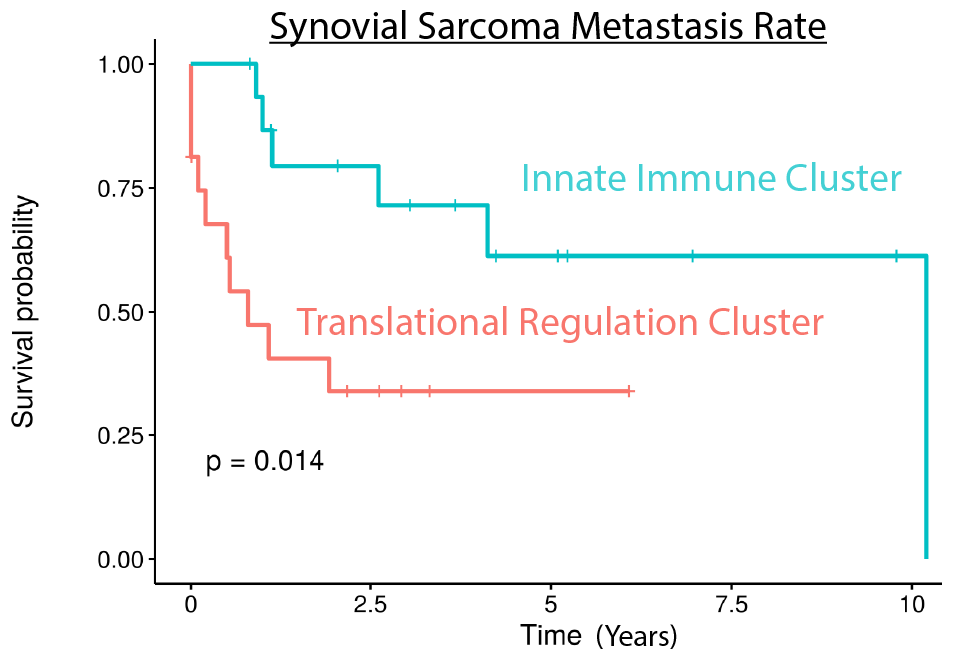
\includegraphics[width=0.75\textwidth]{img/synovial-kaplan-meier-2x}	
\end{table}

\FloatBarrier

%\paragraph*{S1 File.}
%\label{S1_File}
%{\bf Lorem ipsum.}  Maecenas convallis mauris sit amet sem ultrices gravida. Etiam eget sapien nibh. Sed ac ipsum eget enim egestas ullamcorper nec euismod ligula. Curabitur fringilla pulvinar lectus consectetur pellentesque.

%\paragraph*{S1 Video.}
%\label{S1_Video}
%{\bf Lorem ipsum.}  Maecenas convallis mauris sit amet sem ultrices gravida. Etiam eget sapien nibh. Sed ac ipsum eget enim egestas ullamcorper nec euismod ligula. Curabitur fringilla pulvinar lectus consectetur pellentesque.

%\paragraph*{S1 Appendix.}
%\label{S1_Appendix}
%{\bf Lorem ipsum.} Maecenas convallis mauris sit amet sem ultrices gravida. Etiam eget sapien nibh. Sed ac ipsum eget enim egestas ullamcorper nec euismod ligula. Curabitur fringilla pulvinar lectus consectetur pellentesque.

%\paragraph*{S1 Table.}
%\label{S1_Table}
%{\bf Lorem ipsum.} Maecenas convallis mauris sit amet sem ultrices gravida. Etiam eget sapien nibh. Sed ac ipsum eget enim egestas ullamcorper nec euismod ligula. Curabitur fringilla pulvinar lectus consectetur pellentesque.

\section*{Acknowledgments}
We would like to thank the patients and families who participated in translational genomics research. We thank St. Baldrick's Foundation, California Precision Medicine Initiative, National Human Genome Research Institute of the National Institutes of Health for funding support.

\nolinenumbers

% Either type in your references using
% \begin{thebibliography}{}
% \bibitem{}
% Text
% \end{thebibliography}
%
% or
%
% Compile your BiBTeX database using our plos2015.bst
% style file and paste the contents of your .bbl file
% here. See http://journals.plos.org/plosone/s/latex for 
% step-by-step instructions.
% 

\bibliographystyle{plos2015.bst}
\bibliography{zotero-library.bib}

\begin{thebibliography}{10}
% Copy and paste bbl
\end{thebibliography}



\end{document}

